\documentclass[11pt,a4paper,titlepage]{book}
\usepackage[a4paper, headheight=13.6pt]{geometry}
\usepackage[utf8]{inputenc}
\usepackage[english]{babel}
\usepackage{biblatex}
\usepackage{csquotes}
\usepackage{booktabs}
\addbibresource{biblio.bib}
\usepackage{graphicx}
\usepackage{svg}
\usepackage{caption}
\usepackage{subcaption}
\usepackage{longtable}
\usepackage{wrapfig}
\usepackage{geometry}
\usepackage{amsmath}
\usepackage{pgf}
\renewcommand{\vec}[1]{\mathbf{#1}}
\usepackage[hidelinks]{hyperref}
\geometry{a4paper,top=3cm,bottom=3cm,heightrounded,bindingoffset=5mm}
\usepackage{fancyhdr}
\pagestyle{fancy}
\fancyhf{}
\rhead{Università del Piemonte Orientale}
\lhead{Masters Degree Thesis}
\cfoot{\thepage}
\renewcommand*\contentsname{Index}

\begin{document}

\begin{titlepage}
  \voffset=8mm

   \begin{center}
     \includesvg[width=0.50\textwidth]{imgs/logo_upo.svg}
    
      \vspace*{2cm}

      \LARGE{Dipartimento di Scienze e Innovazione Tecnologica}

      \vspace*{0.5cm}

      \LARGE{\bf Corso di Laurea Magistrale in Informatica}
 		
      \vspace*{3cm}

 		  \Large{Masters Degree Thesis}

      \vspace*{0.3cm}

      \Huge{CleanAir Project: a Neural Network approach to cities pollution monitoring}

      \vspace{25mm}
      
      \begin{tabular*}{\textwidth}{l @{\extracolsep{\fill}} l}
        \large{\bf Relatore:} & \large{\bf Candidato:}\\
        \large{Prof. Luigi Portinale} &  \large{Alessandro Abluton} 
      \end{tabular*}
 
       \vfill
 
      \large{\bf Academic Year 2020/2021}
   \end{center}

\end{titlepage}

\thispagestyle{plain}
\begin{center}
    \textbf{Abstract}
\end{center}
COMPLETAMENTE DA RIVEDERE, LO SCRIVERO' ALLA FINE.
\tableofcontents

\newpage
\thispagestyle{plain}

\chapter{Introduction}
This thesis project has been initially inspired by my participation to the 2017 Climathon in Alessandria, a hackaton whose focus is on proposing new ideas to help fighting climate change; in that event I had the first intuition that eventually brought this project to life: "Having a single value of pollution for a whole city is not descriptive enough but to have multiple values for different areas of the urban perimeter would require too much monitoring stations!"
\newline
So I came up with the idea of using a little number of cheap monitoring stations that could move around the city everyday, and the municipal vehicles are perfect carriers for these stations, because they travel across the urban perimeter multiple times per day by doing their normal jobs. After gathering all data, I'm proposing a new way of handling them: use a Deep Convolutional Neural Network and a Multilayer Perceptron to predict pollution at different time agglomerations at any given zone in a city.

\section{Brief introduction to Artificial Intelligence and Deep Learning}
Deep Learning is actually a subset of Artificial Intelligence techniques that focus on Deep Neural Networks, which are particular structures capable of approximating mathematical functions by imitating the really complex neural connections that govern our brain. That being said, Deep Learning is a much specific bit of the whole world of Artificial Intelligence, which is made up by a lot different techniques each with it's own advantages and disadvantages, it is therefore mandatory to first introduce some of the more traditional methods available.

\subsection{The concept of Intelligence}
Before actually starting to talk about Artificial Intelligence we must define the concept of "intelligence" for humans, because our goal is to give computers some form of intelligence. Let us consider a newborn baby: everything he/she sees it's new, never seen before, how will the baby be able to learn?
\newline
\newline
The answer is simply through experience, the old statement \textit{"we learn through our mistakes"} has never been more true because what the newborn does is actually failing a lot and then learning to associate the action \textbf{A} that brought to a bad outcome \textbf{O} to something bad (e.g. a penalty \textbf{P}) therefore he/she will be less prone in the future to repeat the action that brought failure.

Let us look at a real-world example: said newborn sees the kitchen's fires lit for the first time, his/her mother isn't there at the moment so the newborn decides to touch the fire. He/She gets hurt, mommy comes immediately and after healing the wound tells to his baby not to do it again in the future.
When does the \textbf{learning} actually happens? every time the newborn does an action that has a bad outcome, the neural connections that brought his/her brain to perform A become less likely to be activated, as if a penalty P is applied in some form on those connections; in this particular example the action is to touch the fire, the sad outcome are wounds, and the penalty is made up by both the pain and the mother's speech about how the fire is dangerous.
\newline
\newline
The whole challenge of Artificial Intelligence is to enable this process of learning, meaning that we want our software to be less likely to perform an action with some bad outcome; to achieve this goal a software has to know both how much it failed and how to correct itself. 
A lot of different mathematical techniques can be used to achieve this result and most of them have nothing in common, but the goal of each one is exactly the same and is well summarized in a definition of Intelligent Software given by Tom Mitchell \cite{mitchell}:
\newline
\newline
\textit{"A computer program is said to learn from experience \textbf{E} with respect to some class of tasks \textbf{T} and performance measure \textbf{P}, if its performance at tasks in \textbf{T}, as measured by \textbf{P} improves with experience \textbf{E}."}
\newline
\newline
Let us analyze each component of this definition:
\begin{itemize}
    \item \textbf{T}: a class of tasks (or problems) such as Classification, Regression, Clustering
    \item \textbf{P}: some measure of performance, each task has it's most suitable ones 
    \item \textbf{E}: the experience, meaning some time that needs to pass in which the learning software actually learns how to handle it's assigned task, hopefully reaching the optimal solution
\end{itemize}
The experience E is the actual process of trying an action, evaluating it's outcome and adapting the system accordingly reiterated over and over in time until some form of goal is reached, for example in Regression tasks frequently the Mean Squared Error is used as measure of performance and therefore the goal to reach could be that value, calculated between the system's predicted values and the original ones, falling beneath a threshold $\epsilon$.

Having this kind of goal means that we're making a strong assumption: \textit{"Repeating the process of trying some action over time, while slightly changing said action in each iteration, will eventually lead to lower the MSE value"}, but what guarantees do we have that the system is going to tweak the action in a good way, one that will lead to low MSE values, or more generally good values on any kind of performance metric?
\newline
\newline
To tweak an action in a proper way the system needs to actually \textbf{learn} over time how to handle it's task, exactly like the baby newborn does, and that goal is achieved through the help of some sort of \textbf{loss function}, which is a function that is able to tell the system how much it is mistaking. 
Those components are the "building blocks" through which we can analytically describe every problem, and describing a problem is always the starting point to actually solve it.
\newline
\newline
Once understood this concept we can think of Artificial Intelligence as a set of techniques that, through mathematical tricks, try to give computers the ability to "learn from experience" exactly as humans do; so that if an action A is executed in the context of a task T, the measures of performance P let the system correct itself based on A's outcome evaluation.

The experience E is the actual process of trying an action, evaluating it's outcome and adapting the system accordingly, reiterated over and over in time until some form of goal is reached (e.g. the MSE value falls beneath a threshold $\epsilon$).

\subsection{Different learning methods}
\begin{figure}[ht]
    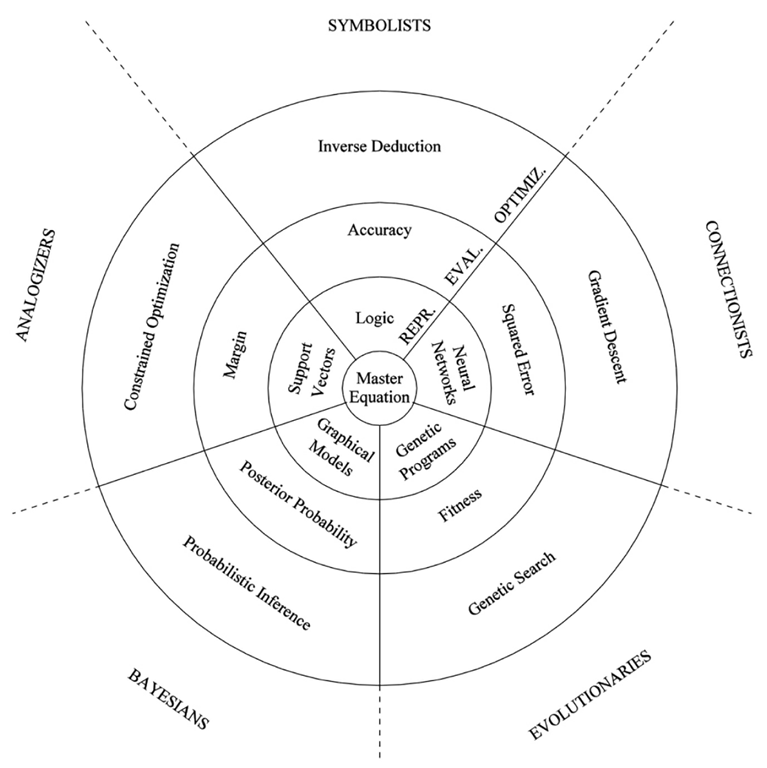
\includegraphics[scale=0.55]{imgs/ch_1/master_algo_ontology.png}
    \centering
    \caption{Domingues's ontolgy for AI methods}
    \label{master_algo_ontology}
\end{figure}
There are a lot of different methods to achieve the goal of having a system capable of learning over time, each with it's own peculiarities. I like to use an ontology written by Pedro Domingues \cite{master_algo}, who splits all these different methods in five tribes, depicted in Figure \ref{master_algo_ontology}:
\begin{enumerate}
    \item The Symbolists. They focus on the premise of inverse deduction: they don’t start with a premise to work towards conclusions, but rather use a set of premises and conclusions and work backward to fill in the gaps.
    \item The Connectionists. They mostly try to digitally re-engineer the brain and all of its connections in a neural network. The most famous example of the connectionist approach is what is commonly known as ‘Deep Learning’. Their techniques have proved very efficient in e.g. image recognition and machine translation.
    \item The Evolutionaries. Their focus lies on applying the idea of genomes and DNA in the evolutionary process to data processing: their algorithms will constantly evolve and adapt to unknown conditions and processes.
    \item The Bayesians: Bayesian models will take a hypothesis and apply a type of “a priori” thinking, believing that there will be some outcomes that are more likely. They then update their hypothesis as they see more data.
    \item The Analogizers: This machine learning discipline focuses on techniques to match bits of data to each other. Probably the most famous example of this type of machine learning, is the Amazon or Netflix recommendations: “If you have watched/bought this, you will probably like…”.
\end{enumerate}
Domingues claims that the ultimate goal of Aritificial Intelligence is to find a Master Algorithm, one that could be able to optimally solve any given task, that's why in Figure \ref{master_algo_ontology} we can see in the center the "Master Equation". 
\newline
\newline
Each one of these methods has seen bot successes and failures over time, and has it's own peculiarities. In this thesis I'm focusing on Neural Networks, the Connectionist's building block to achieve the goal of having a learning system.

\subsection{Neural Networks}
In it's most generic acceptation a Neural Network is mathematical model that tries to reproduce the human brain's cognitive functions by mimicking the actual neural networks inside of it.

The \textit{basic unit} of these networks are the so called \textit{artificial neurons}, which can be seen as structures that receive some input and fire an output if the weighted sum of it's input overcomes a threshold $\epsilon$. 
\newline
\newline
An artificial neuron could be thought of as a "digital representation" of an actual neuron in our brain; as seen in Figure \ref{neuron_med} a real neuron cell receives input through it's dendrites in the form of electrical signals and processes it, if the combination of all the signals it is receiving through it's dendrites is high enough it will fire a signal through the axon, that signal will become an input signal for all the neurons connected to that axon's terminal.
\begin{figure}[ht]
    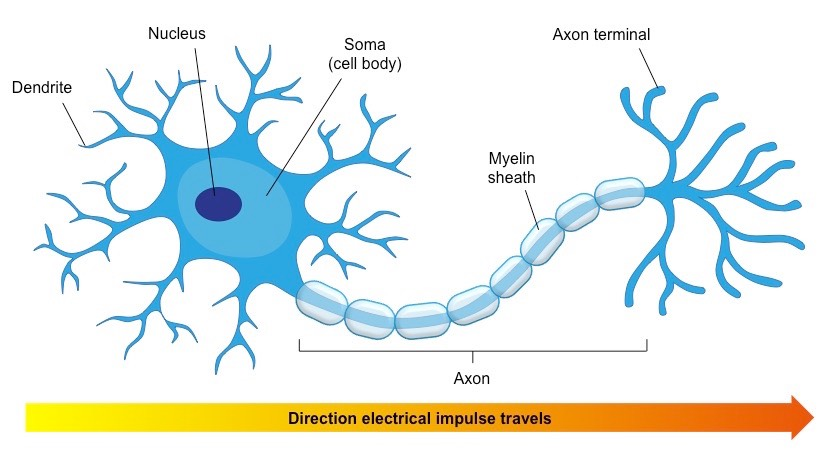
\includegraphics[scale=0.45]{imgs/ch_1/neuron_med.jpeg}
    \centering
    \caption{Simple representation of a neuron cell}
    \label{neuron_med}
\end{figure}
\subsubsection{Rosenblatt's Perceptron}
From the early 1940s a lot of different implementations of a digital neuron have been proposed, one that has become universally accepted is the Single Layer Perceptron proposed by Frank Rosenblatt in 1958 \cite{Rosenblatt1958ThePA}.

In that model the neuron is represented as in Figure \ref{digital_neuron}, it receives an array $x$ of inputs, each element of $x$ has it's weight $w_i$ and there's also a bias parameter $w_0$ that helps in regularizing the model's outputs. Rosenblatt uses also a \textbf{linear activation function} $out(t)$, which represent the threshold value above mentioned; the neuron computes a weighted sum of it's inputs, the passes the result to the activation function: if the value is high enough and passes the threshold the whole neuron will fire a 1 ($out(t)=1$), otherwise it won't fire anything ($out(t)=0$).
\begin{align}
    \begin{cases}
        0   &   \text{if out(t)} < \epsilon \\
        1   &   \text{if out(t)} \geq \epsilon
    \end{cases}
\end{align}

\begin{figure}[h]
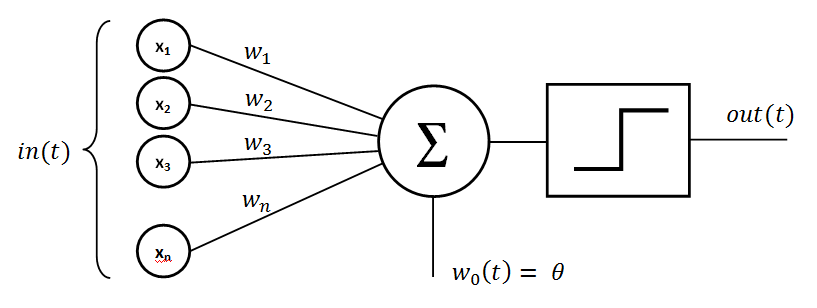
\includegraphics[scale=0.3]{imgs/ch_1/digital_neuron.png}
    \centering
    \caption{Rosenblatt's representation of an artificial neuron}
    \label{digital_neuron}
\end{figure}
The first proposed network by Rosenblatt consisted only in one single neuron as depicted in Figure \ref{digital_neuron}, but even if it's underlying concept was mathematically strong and trusted it wasn't able to approximate functions with sufficient precision, mostly because the fact of having a linear activation function makes it able to approximate well only linear functions, and it hardly happens that a real-world problem can be solved by such functions. This weakness is the reason why it never grew so much interest in the scientific community at it's earliest stages.

\subsubsection{Multilayer Perceptron}
The next advancement was made by creating an actual network of neurons known as Multilayer Perceptron (Figure \ref{mlp_example}), which greatly improved the approximation capabilities of these models. 
\begin{figure}[h]
    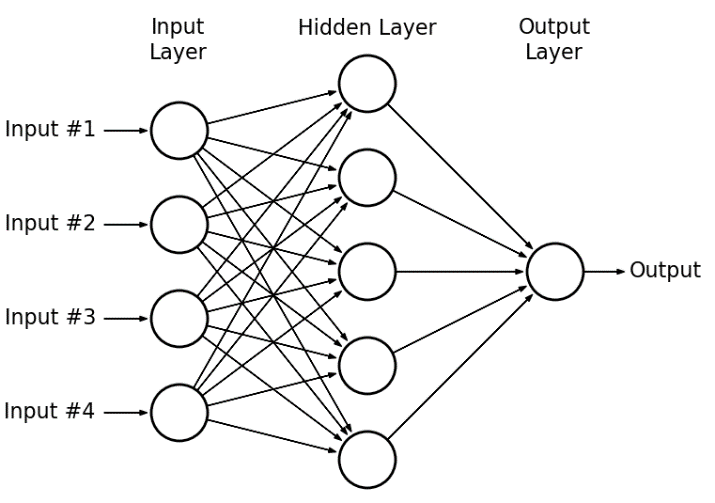
\includegraphics[scale=0.4]{imgs/ch_1/A-hypothetical-example-of-Multilayer-Perceptron-Network.png}
    \centering
    \caption{An example of Multilayer Perceptron}
    \label{mlp_example}
\end{figure}
The network is made up by three layers of neurons, with the hidden layer that usally has more neurons than the input layer and the output one that is either made up by a single neuron for regression task, or by $n$ neurons for n-class classification tasks (meaning that the i-th output neuron holds the probability that the j-th sample belongs to class i).
\newline
\newline
This added complexity gives the model the ability of approximating \textit{non-linear functions} because every hidden layer is actually defining an hyperplane intersected with input data's vector space. The splitting of that space in more and more complex regions lets the system describe at best the values of input data.
\subsubsection{Perceptron's learning algorithm}
Mathematically speaking, learning for a single Perceptron (or neuron) means tweaking the weights \textbf{w} associated to the inputs \textbf{x} so that the hyperplane generated by the weighted sum of inputs and weights will separate linearly the input data in the best possible way.

To achieve that goal we use the difference between the correct value and the one produced by the network: the grater the error, the more weights tweaking still needs to be done in order to obtain the best possible hyperplane. 
\newline
Given a set of weights \textbf{w} and a set of inputs \textbf{x}, the value of i-th weight will be modified with this formulae:
\begin{align}
    w_i = w_i + \eta E x_i \\
    E = (t - y(x))
\end{align}
$E$ represents the error between the original value $t$ and the network's produced one $y(x)$ and it is referred to as \textit{loss function}, while $\eta$ is a constant known as \textit{learning rate} with values in range $[0, 1]$ used to set a value to tweak the weights with, the closer to 1 the higher are the changes be made to said weights.
\newline
\newline
Setting a proper learning rate is mandatory to get good results, both in terms of training speed and prediction's accuracy; as seen in Figure \ref{learning_rate}, if set too close to 1 the weights will be changed too much in each iteration and there will be a high risk of completely missing an actual minimum, whereas if set to close to 0 the learning process would be really accurate but tremendously slow and therefore infeasible in terms of time and money.
\newline
\newline
Assuming that the set of input samples is linearly separable and $\eta$ is small enough, this kind of learning will always eventually converge.
\begin{figure}[ht]
    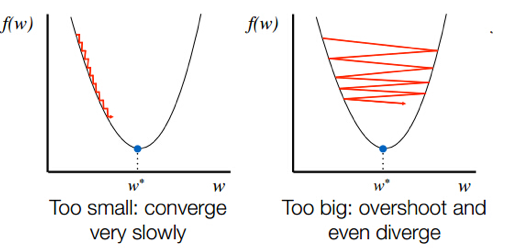
\includegraphics[scale=0.60]{imgs/ch_1/learning_rate.png}
    \centering
    \caption{Learning rate problem}
    \label{learning_rate}
\end{figure}
\subsubsection{Multilayer learning, Gradient Descent}
The main goal of this method is reaching the lowest possible value of some loss function, by using the best values for the weights vector \textbf{w}. The weights are modified in accordance to the loss function's minimum, calculated by deriving said function in respect to each component of \textbf{w}:
\begin{align}
    w_i = w_i + \Delta w_i \\
    \Delta w_i = - \eta \frac{\partial E}{\partial w_i} \\
    E = \frac{1}{k} \sum_{i=1}^{k}(t_i - y(x_i))^2 \\
    y(x) = \sum_{i=1}^{k}x_i w_i
\end{align}
The learning rate is a positive constant but as we can see in (1.5) it is negated, because the goal is to reach the \textit{lowest} value of $E$.
\newline
The loss function used in this example $E$ is the Mean Squared Error, but actually any function that is able to give a form of error works, the difference is in what kind of error we are considering: different loss functions produce different trained models because each one gives more importance to different aspects of the prediction error. 

To further clarify let us consider the Mean Squared Error, given the fact that every error gets squared by using this kind of function we are penalizing large mistakes much more than the small ones, an error of 200 means an MSE of 40000, where an error of 0.1 produces an MSE of 0.01. 
\newline
\newline
The \textbf{Gradient Descent Algorithm} is the process of repeating this operation over and over in time, until some goal is reached; usually it could be a fixed number of iterations to perform, the loss function reaching a fixed value, but any kind of stopping criteria can be experimented.

\subsection{Convolutional Neural Networks}
There are a lot of different models of neural networks, each with it's best use case; given that in this thesis I'm making use of map images to predict pollution levels I focused my work upon Convolutional Neural Networks, the state-of-the-art model for all kinds of computer vision tasks.
\newline
\newline
Convolutional networks (LeCun, \cite{lecun-bengio-95a}) also known as CNN, are a particular model of neural network capable of handling data known to have a grid-like topology such as time series (can be thought as a 1-D grid of all the samples taken at regular time intervals, or images (2-D grid of pixels).

These networks are one of the main reason why Deep Learning gained so much interest in recent times, thanks to the amazing results achieved in computer vision tasks (e.g. handling of images and video related tasks) a lot of which are actually shaping the new society of this century.

One of the most iconic examples is the chinese government's model for Facial Recognition:  in 2018 it reached almost perfection with values of accuracy as high as 95\% (human accuracy is estimated to be $~93\%$) in this task thanks to the really complex and powerful surveillance system spread country-wide. A lot could be argued about the method used by that government to get that much accuracy, but ethical implications regarding these kind of networks are out of the scope of this thesis.
\newline
\newline
An intuitive definition that describes convolutional network is given by Ian Goodfellow \cite{Goodfellow1}: 
\begin{center}
    \textit{Convolutional networks are simply neural networks that use convolution in place of general matrix multiplication in at least one of their layers}
\end{center}
The real game-changing peculiarity of this network is that it actually learns how to extract features from images, so that those features are descriptive enough to make the prediction process as optimal as possible, and as the definition says what makes it possible is the \textbf{operation of convolution}.
\newline
That is because one of the most challenging problems in image recognition tasks is the \textbf{feature extraction}: what features of a dog's picture make it an actual dog picture? what should the model be looking for, to determine whether the image it is analyzing contains a dog, a cat or both of them?
\newline
\newline
A convolutional network is made up by a fixed number of \textit{convolutional layers}, each with the task of extracting different feature sets from an image. The first layers will be the ones that recognize wider features such as contours of things and the last ones will be recognizing patterns and colors that only in appearance have nothing to do with the problem to be solved, but they are actually really useful to get good results.

\subsubsection{The Convolution Operation}
\label{convolution:explanation}
In its most generic abception, convolution is a linear operation on two functions of a real-valued argument, and it is usually denoted with an asterisk:
\begin{align}
    s(t) = \int_{a}^{b} w(y) x(t-y) dy \\
    s(t) = (x*w)(t)
\end{align}
There are differences between the meaning of each component, depending if convolution is used in a classical math context or in convolutional network; in classical math terminology $w(y)$ is a probability density function normalized in $[a,b]$.
\newline
Instead in convolutional networks terminology the first argument $x$ is called the \textbf{input} and the second one $w$ is the \textbf{kernel}, the output of this operation is called \textbf{feature-map} and $t$ is the \textbf{time index}.
In this form it's impossible to take \textit{continue} measures, therefore we must switch to the \textit{discrete} variant of convolution (example for 1-D signals):
\begin{align}
    s(t) = \sum_{k=-\infty}^{+\infty} w(k) x(t-k)    
\end{align}
Usually the input \textbf{x} is a multidimensional array of data and the kernel is a multidimensional array of parameters randomly generated and then subsequently adapted by the learning algorithm, so that the convolution operation highlights the more suitable features of the image.

These kind of multidimensional parameters will be referred to as \textbf{tensors}.
\begin{figure}[ht]
    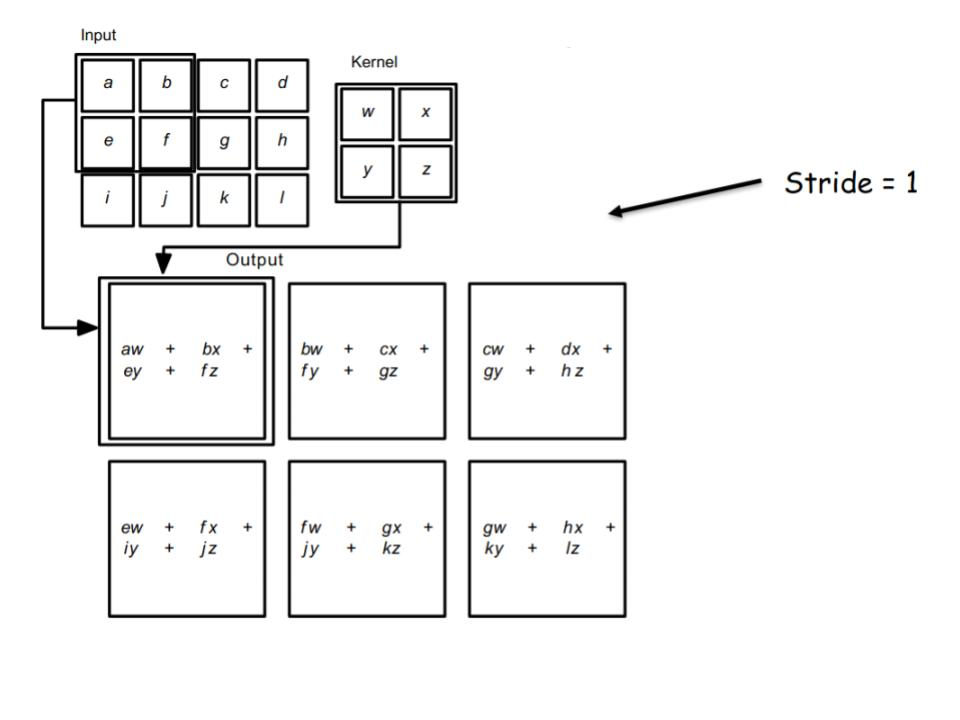
\includegraphics[scale=0.5]{imgs/ch_1/convolution.jpg}
    \centering
    \caption{An example of Convolution on an image, with stride=1: the first time K is applied to the pixels \textit{"a, b, e, f"}, but in the next iteration it will be applied to the pixels \textit{"b, c, f, g"}}
    \label{convolution_example}
\end{figure}
\newline
\newline
When handling images or any kind of 2-D data, the convolution has to be performed on two dimensions:
\begin{align}
    S(i, j) = (K * I)(i, j) = \sum_{m}\sum_{n}I(m,n)K(i - m, j - n)
\end{align}
where I is the intensity value of the pixel in position \textit{(m, n)} in the image and K is the kernel. 
\newline
\newline
Convolution is \textbf{commutative}, therefore (1.11) could be written like this:
\begin{align}
    S(i, j) = (K * I)(i, j) = \sum_{m}\sum_{n}I(i - m, j - n)K(m, n)
\end{align}
usually the latter formula is used in machine learning applications, because the values of \textit{n} and \textit{m} will variate less than the former one.
\newline
\newline
The commutative property of convolution arises because we have flipped the kernel relative to the input, in the sense that as m increases, the index into the input increases, but the index into the kernel decreases.
\newline
It's important to notice that many neural network libraries implement the \textbf{cross-correlation} but call it convolution, which is actually the same but without flipping the kernel:
\begin{align}
    S(i,j) = (I*K)(i,j) = \sum_{m}\sum_{n}I(i+m, j+n) K(m,n)
\end{align}
In any case, the learning algorithm will learn the proper values of the kernel in the right place, so an algorithm based on convolution with kernel flipping will learn a kernel that is flipped relative to the kernel learned by an algorithm without the flipping.

\subsubsection{Why use convolution}
The use of convolution leverages three important concepts: \textbf{sparse interactions}, \textbf{parameter sharing}, \textbf{equivariant representations}, and it also provides a convenient way of dealing with inputs of variable size.
\newline
In traditional neural networks \textit{every output unit interacts with every input unit}, while convolutional networks tipically have sparse interactions (also referred to as \textbf{sparse connectivity} or \textbf{sparse weights}). This is caused by the kernel being much smaller than the input, and that gives the ability to detect small and meaningful features (that occupy only a few thousands pixels) such as edges, corner or particular patterns.
For a graphical representation of sparse interaction see Figures \ref{sparse_connectivity_above} and \ref{sparse_connectivity_below}. This idea means that it's not anymore necessary to hold all the network's parameters at once, which both improves statistical efficiency and lowers the memory requirement.
\newline
\newline
\textbf{Parameter sharing} refers to using the same parameter for more than one function in a model, while in traditional networks each parameter is used only one time when computing the output of a layer. In convolutional networks each element of the kernel is used at every position of the input (except perhaps the boundaries of the image); this means that rather than learning a single set of parameters for every location, and that reduces even more the storage requirements to \textit{k} parameters. 

See Figure \ref{parameters_sharing} for a representation of parameter sharing in action.
\newline
\newline
The specific form of parameter sharing used in this networks causes the layers to have a property called \textbf{equivariance to translation}. A function is equivariant when if its input changes, the output changes in the same way: $f(g(x)) = g(f(x))$, and in the context of convolution this means that input and output of a layer are changing in the same way.
\newline
\newline
Practically speaking, when dealing with 2-D data like images convolution produces a \textbf{feature map} which is basically a map of where certain features appear in the image; if we move the object in the input its representation will move by the same amount in the output, so it's really useful to share parameters through the deeper layers of the network.

As an example, when the first layer detects edges it is really useful to share those parameters across the network because that same small edge will appear in a lot of different parts of the image.

\begin{figure}[ht]
    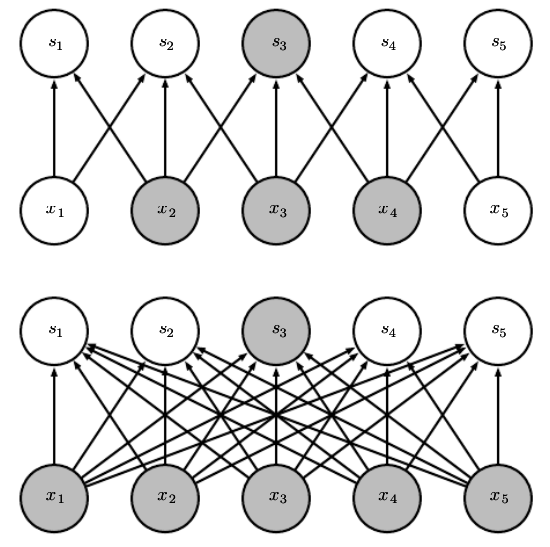
\includegraphics[scale=0.5]{imgs/ch_1/sparse_connectivity.png}
    \centering
    \caption{Graphical representation of \textit{sparse connectivity from above}: the convolution with a kernel of size 3 gets the highlighted $s_3$ output unit to be connected only to input units $x_2$, $x_3$, $x_4$, in both networks the highlighted units form the \textbf{receptive field} of $s_3$}
    \label{sparse_connectivity_above}
\end{figure}
\begin{figure}[ht]
    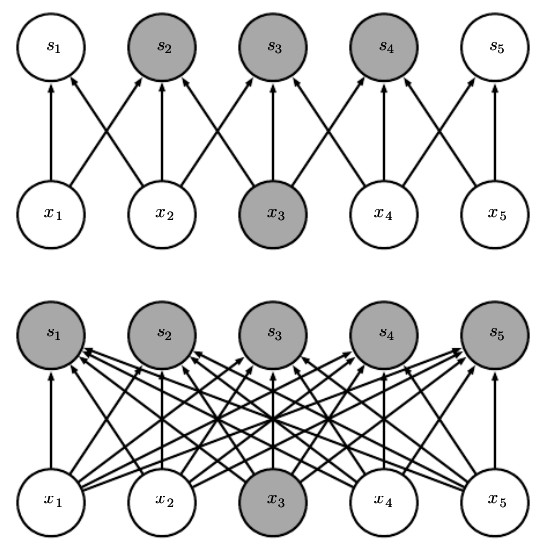
\includegraphics[scale=0.5]{imgs/ch_1/sparse_connectivity_below.png}
    \centering
    \caption{Graphical representation of \textit{sparse connectivity from below}: when convolution is performed with a kernel of size 3 the input unit $x_3$ is connected only to output units $s_2$, $s_3$, $s_4$}
    \label{sparse_connectivity_below}
\end{figure}
\begin{figure}[ht]
    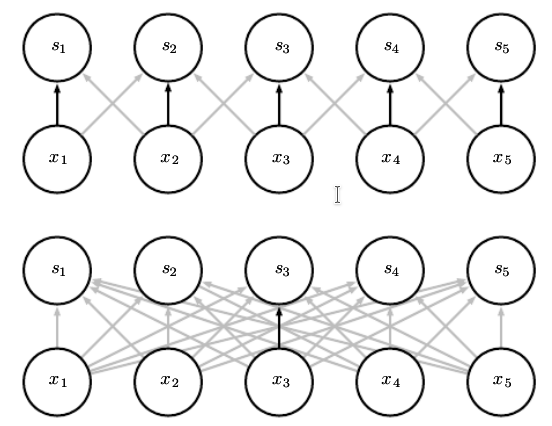
\includegraphics[scale=0.5]{imgs/ch_1/parameter_sharing.png}
    \centering
    \caption{Graphical representation of \textit{parameters sharing}: the arrows indicate the connections that use a particular parameter in both models. In convolutional networks thanks to parameter sharing only the kernel's parameters are shared between units}
    \label{parameters_sharing}
\end{figure}

\subsection{Pooling}
A typical layer of a convolutional network consists of three stages (see Figure \ref{cnn_schema}):
\begin{enumerate}
    \item The first stage is called \textbf{convolutional stage} and performs several convolutions in parallel to produce a set of linear activations.
    \item The second one is sometimes called \textbf{detector stage} and runs each linear activation through a nonlinear activation function, such as the rectified linear activation function.
    \item The last stage is called \textbf{pooling stage} and uses a pooling function to further modify the layer.
\end{enumerate}
A \textbf{pooling function} replaces the output of the network at a given location with some sort of statistic summary of the nearby outputs; let us consider the \textbf{max pooling function} as an example: this operation reports the maximum output value within a rectangular window (Zou and Chellappa, 1988).
\begin{figure}[ht]
    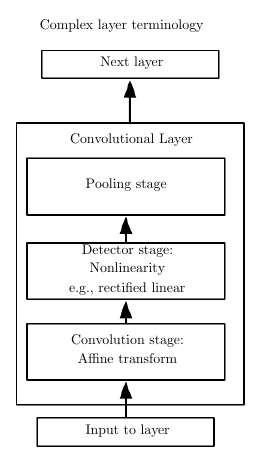
\includegraphics[scale=0.5]{imgs/ch_1/cnn_schema.png}
    \centering
    \caption{A schema of a typical convolutional neural network layer, usually the network is seen as a small number of complex \textit{convolutional layer}, each one made up by a \textit{convolution stage} followed by a stage that introduces nonlinearity called \textit{detector stage} and in the end there's the \textit{pooling stage} that shrinks the output to smaller dimensions}
    \label{cnn_schema}
\end{figure}
Independently from the pooling function used, this stage helps to make the representation become approximately \textbf{invariant} to small translations of the input. Invariance to local translations can be a very useful property if one cares more about whether some features are present in the image than exactly knowing their position.
\begin{figure}[ht]
    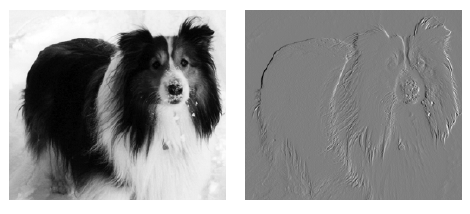
\includegraphics[scale=0.5]{imgs/ch_1/feature_map.png}
    \centering
    \caption{An example of \textit{edge detection}: the image on the right was formed by taking each pixel in the original image and subtracting the value of its neighbouring pixels on the left}
    \label{feature_map}
\end{figure}

\subsubsection{Kernel learning, Backpropagation of the error}
The feature extraction is made by the convolution between the image and a kernel. What a convolutive network learns is actually how to find the best values for the kernel so that the best representative features are extracted.
\newline
\newline
If we consider the values of the kernel as weights to learn, it becomes possible to use any kind of learning algorithm already used for traditional networks, for the goal is always the same: \textit{minimize the loss function by modifying the weights of the network}.
\newline
\newline
The most important learning algorithm for neural networks based on gradient optimization is called \textbf{backpropagation}. This technique modifies the weights of the network backwards, from the output to the input, so that after calculating the loss function all the weights of the former layers will be updated in accordance to the error.

Backpropagation is an efficient method based on minimization of the loss function, therefore what it actually does is calculating the partial derivatives of each parameter of the network in order to apply a Gradient Descent Algorithm on the network.
\newline
It uses the \textbf{chain rule} to calculate the derivative of a composite function, keep in mind that each activation can be seen as a composite function made up by all the linear combination in input to its unit. 
\newline
\newline
Let us consider a network with a single input unit, one hidden unit and one output: the derivative of the loss function against the weights to modify can be written as follows:
\begin{align}
    E(\sigma(z)), z = x_i * w_i \\
    \frac{\partial E}{\partial w_i} = \frac{\partial E}{\partial \sigma} \frac{\partial \sigma}{\partial z} \frac{\partial z}{\partial w_i}
\end{align}
This exact method can be used to modify the kernel's weights in accordance to the cost function. Assuming that:
\begin{itemize}
    \item $x_{i,j}^l \longrightarrow$ it's the result of convolution stage at layer \textit{l}
    \item $w_{m,n}^l \longrightarrow$ are the weights of the kernel used at layer \textit{l}
    \item $o_{i,j}^l \longrightarrow$ it's the nonlinear activation function of layer \textit{l}, executed on the output of convolution ($o_{i,j}^l = ReLU(x_{i,j}^l)$)
    \item $b_l \longrightarrow$ is the bias for layer \textit{l}
    \item $H x W \longrightarrow$ are the dimensions of the feature map produced by the layer
    \item $K1 x K2 \longrightarrow$ are the dimensions of the kernel
\end{itemize}
it becomes possible to formally prove how to calculate the variation to apply for every single pixel of a kernel:
\begin{align}
    \frac{\partial E}{\partial w_{m',n'}^l} = \sum_{i=0}^{H-k_1} \sum_{j=0}^{W-k_2} \frac{\partial E}{\partial x_{i,j}^l} \frac{\partial x_{i,j}^l}{\partial w_{m',n'}^l}
\end{align}
In (1.16) $x_{i,j}^l$ is equivalent the result of the convolution performed between the kernel K for the layer \textit{l} and the feature map produced by the previous layer \textit{l-1}, so it could be written as $x_{i,j}^l = \sum_{m}\sum_{n} w_{}^l o_{i+m,j+n}^{l-1} + b^l$. By expressing $x_{i,j}^l$ in terms of convolution we get:
\begin{align}
    \frac{\partial x_{i,j}^l}{\partial w_{m',n'}^l} = \frac{\partial}{\partial w_{m',n'}^l} ( \sum_{n} \sum_{n} w_{m',n'}^l o_{i+m,j+n}^{l-1} + b^l )
\end{align}
The partial derivative is zero everywhere except for the one with indexes $m = m'$ and $n = n'$, therefore the output will be the pixels of the features map produced in layer \textit{l-1} associated with the pixels of the kernel at level \textit{l}:
\begin{align}
    \frac{\partial x_{i,j}^l}{\partial w_{m',n'}^l} = \frac{\partial}{\partial w_{m',n'}^l} (w_{0,0}^l o_{i+0, j+0}^{l-1} + \dots + w_{m',n'}^l o_{i+m', j+n'}^{l-1} + \dots + b' )
\end{align}
After deriving, the weights with indexes $m'$, $n'$ will become 1, therefore considering that every weight except those two becomes zero only the activation will remain: $o_{i+m', j+n'}^{l-1}$. 
\newline
The last term of (1.16) to be calculated is $\frac{\partial E}{\partial x_{i,j}^l}$, that represents the actual error to backpropagate through the network and will be referred to as $\delta_{i,j}^l$:
\begin{align}
    \delta_{i,j}^l = \frac{\partial E}{\partial x_{i,j}^l}
\end{align}
this value states the variation of the pixel $i,j$ in the feature map $o^{l-1}$ in respect to the loss function. By applying the \textbf{chain rule} we obtain:
\begin{align}
    \frac{\partial E}{\partial x_{i',j'}^l} = \sum_{m=0}^{k_1-1} \sum_{n=0}^{k_2-1} \frac{\partial E}{\partial x_{i'-m,j'-n}^{l+1}} \frac{\partial x_{i'-m,j'-n}^{l+1}}{\partial x_{i',j'}^l} = \sum_{m=0}^{k_1-1} \sum_{n=0}^{k_2-1} \delta_{i'-m,j'-n}^{l+1} \frac{\partial x_{i'-m,j'-n}^{l+1}}{\partial x_{i',j'}^l} 
\end{align}
By subtracting the kernel's indexes to the ones of the feature map ($i'-m,j'-n$) we obtain the points influenced by the previous layer within the region of convolution. Intuitively the a pixel that's an inpu for layer \textit{l} will influence the value of much more pixels in the features map that goes in input to layer \textit{l+1}. 
\newline
The term $x_{i'-m,j'-n}^{l+1}$ represents the output of layer \textit{l+1}, therefore it can be written as the convolution between the output of layer \textit{l} and the kernel of layer \textit{l+1}:

\begin{align}
   \notag \frac{\partial x_{i'-m,j'-n}^{l+1}}{\partial x_{i',j'}^{l}} = \frac{\partial}{\partial x_{i',j'}^{l}} \left( \sum_{m'} \sum_{n'} w_{m',n'}^{l+1} o_{i'-m+m', j'-n+n'} + b^{l+1} \right) \\ 
   = \frac{\partial}{\partial x_{i',j'}^{l}} \left( \sum_{m'} \sum_{n'} w_{m',n'}^{l+1} f(x_{i'-m+m', j'-n+n'}^l) + b^{l+1} \right) 
\end{align}
In equation (1.21) only the weights with indexes $m',n'$ and the activation functions applied to pixels $i',j'$ will have values, every other term will be equal to zero:
\begin{align}
    \notag \frac{\partial x_{i'-m,j'-n}^{l+1}}{\partial x_{i',j'}^l} = \frac{\partial}{\partial x_{i',j'}^{l}} \left( w_{m',n'}^{l+1} f(x_{0-m+m', 0'-n+n'}^l) + \dots + w_{m,n}^{l+1}f(x_{i',j'}^l) + \dots + b^{l+1}\right) \\
    = \frac{\partial}{\partial x_{i',j'}^{l}} \left( w_{m,n}^{l+1} f(x_{i',j'}^l) \right) = w_{m,n}^{l+1}\frac{\partial}{\partial x_{i',j'}^{l}}\left( f(x_{i',j'}^l) \right) = w_{m,n}^{l+1} f'(x_{i',j'}^l)
\end{align}
The partial derivative of equation (1.20) can be rewritten as:
\begin{align}
    \frac{\partial E}{\partial x_{i',j'}^l} = \sum_{m=0}^{k_1-1} \sum_{n=0}^{k_2-1} \delta_{i'-m, j'-n}^{l+1} w_{m,n}^{l+1} f'(x_{i',j'}^l)
\end{align}
It is now possible to \textbf{formalize backpropagation}:
\begin{align}
    \frac{\partial E}{\partial w_{m',n'}^l} = \sum_{i=0}^{H-k_1} \sum_{j=0}^{W-k_2} \frac{\partial E}{\partial x_{i',j'}^l} \frac{\partial x_{i,j}^l}{\partial w_{m',n'}^l} = \frac{\partial E}{\partial x_{i',j'}^l} \delta_{i,j}^l \frac{\partial x_{i,j}^l}{\partial w_{m',n'}^l}
\end{align}
where $\delta_{i,j}^l$ is obtained via equation (1.23) while $\frac{\partial x_{i,j}^l}{\partial w_{m',n'}^l}$ corresponds to $o_{i+m',j+n'}^{l-1}$. By using the convolution operator $*$ between those two components a matrix will be generated which will calculate the kernel's values when it gets applied to a region of the output feature map.

\section{Why studying climate change?}
The Earth's climate has continuously changed through history, just in in the last 650.000 years there have been seven cycles of glacial advance and retreat; the last ice age ended about 11.700 years ago and set the start of the modern climate era.

The very most part of these changes are considered to be the cause of small variations in our planet's orbit, that consequently change the amount of solar energy the Earth receives.
\newline
\newline
According to the Fifth IPCC assessment report on climate change \cite{ipcc-fifth}, even if there have been cycles in climate change, the current warming trend is of particular significance because it's most likely mankind's fault (with a probability higher than $95\%$), since it started in the mid twentieth century with the first industrial revolution and has continued to grow at unprecedented rates, never seen in history.

Thanks to all the satellites orbiting around our planet, scientist have been able to demonstrate that \textit{carbon dioxide and other pollution-related gases have a heat trapping nature}, their ability to affect the transfer of infrared energy through the atmosphere is the scientific base of many instruments used by NASA. It is therefore safe to say:
\begin{center}
    \textit{There is no question that increased levels of greenhouse gases must cause the Earth to warm in response}
\end{center}
Even if Earth isn't new to climate changes as said before, evidences like ice cores drawn from Greenland or Antarctica, tree rings, ocean sediments, reveal that the current warming is occurring almost ten times faster than the ones happened after ice ages, as seen in Figure \ref{climate_change_nasa}.
\newline
\begin{figure}[ht]
    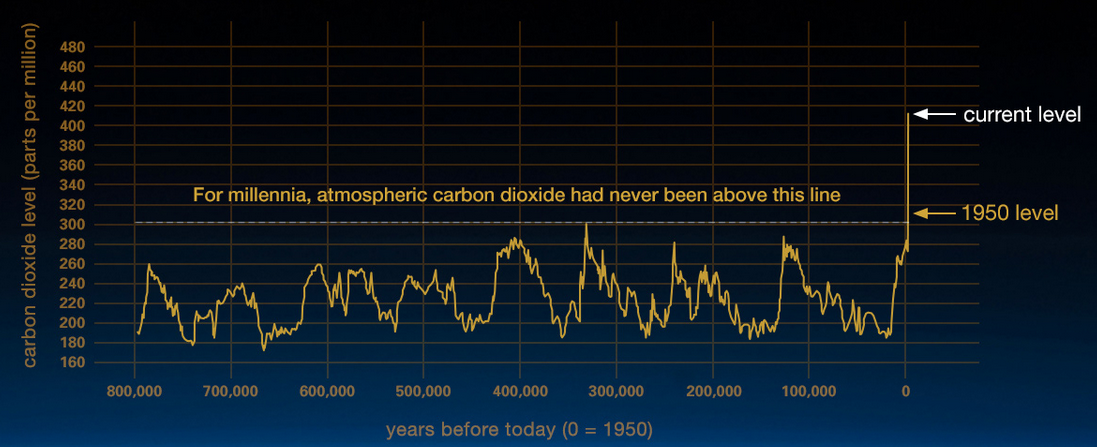
\includegraphics[scale=0.50]{imgs/ch_1/climate_change_nasa_plot.png}
    \centering
    \caption{History of climate change, comparison of both atmospheric samples contained in ice cores and more recent direct measurements; a cyclic trend emerges, the lowest points are the ice ages}
    \label{climate_change_nasa}
\end{figure}
Such an unprecedented increase in temperatures is having observable effects on almost every kind of environment present on Earth: glaciers are shrinking more and more, ice on rivers and lakes disappears sooner than ever, plant and animal ranges have shifted  and even trees are flowering sooner.
\newline
Each one of these consequences could be considered not harmful in itself, but the indirect damages caused are almost unimaginable: for example, loss of sea ice is actually making every sea in the world to rise alarmingly, causing both loss of dry land (fundamental for agriculture and therefore our sustenance) and longer, more intense waves that further accelerate this process.
\newline
\newline
It is now a common belief amongst scientists that global temperatures will continue to rise for decades to come, due to all the greenhouse gases produced by human activities. The Intercontinental Panel on Climate Change (IPCC), which includes more than a thousand of scientists from almost every part of the world, has forecasted a rise of up to 4 degrees Celcius over the next century.

\subsubsection{Climate change affects economy}
According to IPCC's scientists, \textit{the range of published evidence indicates that the net damage costs of climate change are likely to be significant and to increase over time}.
\newline
\newline
Every sector of economy is both the victim and the murderer; in Figure \ref{epa_source_gases} there's a pie plot describing estimates values of how much each sector is responsible for the production of greenhouse gases. Intuitively enough the transportation and electricity sectors are the most impacting ones, mostly because for both of them a large role is still played by burning carbon fossil fuels (over $90\%$ of transports worldwide are still using petroleum based fuels).
\begin{figure}[ht]
    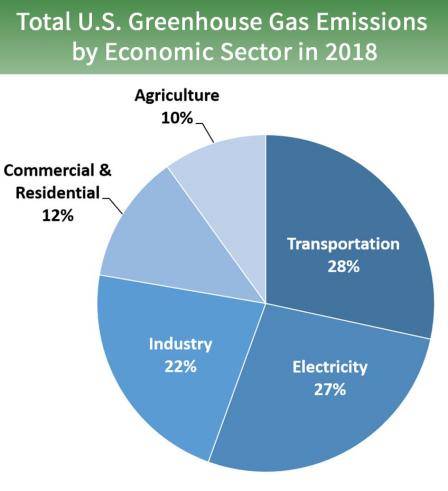
\includegraphics[scale=0.60]{imgs/ch_1/epa_source_gases.jpg}
    \centering
    \caption{Greenhouse gases emissions by economic sector, source USA Environmental Protection Agency. In 2018 a total amount of 6,667 million metric tons of $CO_2$ equivalent has been produced.}
    \label{epa_source_gases}
\end{figure}
\newline
\newline
How will the economy be affected by this changes?
\newline
As said before maybe the biggest risk is the sea level rising due to the increasing temperature, but also the temperature in itself could easily become a problem, because it initiates a chain of bad outcomes:
\begin{enumerate}
    \item Coastal areas are currently being adapted to the increasing sea level
    \item If the forecasting will become real in future, a whole lot of really difficult challenges will arise, such as:
        \begin{itemize}
            \item Relocation of whole towns
            \item Greatly reduced productivity of harvest due to the lack of dry soil
            \item Therefore, prices of basic food will rise exponentially
            \item More wars, to gain possession of the limited resources such as soil and drinkable water
        \end{itemize}
    \item Extreme meteorological phenomena will become more frequent, causing widespread poverty
    \item Higher temperatures will also ease the spread of diseases
\end{enumerate}
Another important factor to consider is that workers worldwide will be more likely to suffer from really bad condition of life, therefore diminishing greatly their productivity. All the health systems worldwide will be overwhelmed and therefore health conditions of individuals will be a great problem in the future.

\subsubsection{How are we fighting?}
The very first cause of climate change is mankind itself: our need for commodity always and everywhere is the main cause. A lot of examples could be made in this regard: we want to have perfect temperature in our houses both in winter (by warming them) and in summer (by cooling them), we use carbon-fueled transports even when a walk could be absolutely feasible, the list could go on and on for a long time, sadly.
\newline
\newline
Luckily in these last years a lot of initiatives carried on by governments, scientists and citizens are quickly rising awareness about this topic.

As an example consider the beautiful project \textit{Fridays for future} founded by Greta Thunberg: even if it's nothing else than public informative events where the topic of climate change is discussed, it brought hundreds of thousands of people (mostly youngsters) together listening to all these facts, and maybe it will bring good changes in everyone's behaviour.
\newline
\newline
The most important change must come from each and every one of us humans; it's mandatory to change our behaviours to a more virtuous standard, otherwise all the efforts made by any organization in the world will have close to none effects.
\newline
There are some technologies that try to capture pollution from the air via complex air filtering techniques, but they surely are too costly to be an actual solution to the problem. Lots of efforts are also being put in developing efficient and accurate methods to monitor pollution worldwide, ranging from satellites to pollution monitoring stations.
\section{CleanAir Project}
CleanAir Project began in December 2017 in the context of a Climathon: an hackaton focused on ideas about fighting climate change, held in thousands of cities across the world each year.
\newline
\newline
I participated to the challenge with a few colleagues from university just for the fun of taking part to an hackaton; we had 24 hours to come up with an innovative idea, make a slideshow and try to convince the judges that your team is the best one.
\newline
\newline
Initially I spent some time in researching news about climate change, with the hope that they would give me good ideas; after a while I came across the problem of monitoring the pollution in cities, a challenge still to overcome due to the lack of both reliable and inexpensive technologies.
\newline
Sadly, climate change is not a problem that affects us at the current time (at least, not with its most severe consequences) and therefore it's highly unlikely that organizations such as governments will ever be positive in spenging lots of money in this regard, and that's why I thought that one of the key concepts in my idea should have been the inexpensiveness.
\newline
\newline
The biggest constraint to monitoring large territories is that a large number of monitoring stations is needed, due to the fact that air (and the particles it contains) moves around because of the wind and any other weather factor. But handling large numbers of stations is not a feasible challenge to anyone, not only due to the cost of actually building and deploying lots of stations, but also due to the fact that each station will require maintenance as time passes by.
\newline
\newline
Then I also thought that in Artificial Intelligence \textit{the power lies in the numbers}, meaning that usually the only constraint is that a lot of data is needed to let the system learn; therefore I came up with the idea behind CleanAir Project: \textit{Using a small number of \textbf{mobile} monitoring stations, mounted on top of municipal vehicles}.

By placing the mobile stations on top of the municipal vehicles the problem of having lots of static stations falls, because those vehicles (coaches, police cars, any kind of service vehicle actually) are used by the workers whom by doing their job will eventually cover the city perimeter, therefore greatly reducing the number of needed stations.
\newline
\newline
Me and my colleagues implemented this idea, thanks also to the help of the University and some professors who provided help and resources as much as they could, in the context of a national challenge organized by CINI (Comitato Interuniversitario Nazionale per l'Informatica).

The challenge was called CINI Smartcities 2018 and as the name suggests, the idea was having teams of undergraduates challenging each other with actual implementations of ideas in the field of Computer Science applied to Cities.
\newline
CleanAir was presented at the challenge in combination with FireStop, another environmental project developed by other colleagues; after some rounds of selections, the challenge ended at the Gran Sasso Science Institute (L'Aquila, Abruzzo, Italy) where me and my team got the second place amongst 15 other Italian universities, thanks to the combination of CleanAir Project and Firestop.
\newline
\newline
Also, this thesis was accepted to participate in CINI 2019 Ital-IA \cite{Ital-IA} conference, where all Italian researchers and research groups on Artificial Intelligence presented what they were working on; even if this is an undergraduate thesis I have been accepted to the conference and given a 10 minute speech to explain what I was working on, it has been a truly wonderful experience.
\subsection{App architecture}
\label{cleanair:apparch}
The application has three major modules:
\begin{itemize}
    \item Data gathering
    \item Data analysis and storage
    \item Data visualization
\end{itemize}
we'll now analyze and explain each module in depth, to show how all these tasks are accomplished. A high-level view of the app's architecture is shown in Figure \ref{cleanair_schema}. 
\begin{figure}[ht]
    \centering
    \includesvg[scale=0.60]{imgs/ch_1/CleanAir_schema.svg}
    \caption{High-level schema of CleanAir Project architecture}
    \label{cleanair_schema}
\end{figure}
\subsubsection{Data gathering}
This module includes both how the stations work and how to gather data from the monitoring stations and send them to the cloud; it is accomplished by means of the MQTT protocol used in Mosquitto's implementation.
\newline
\newline
Figure \ref{cleanair_station} shows a schema of the station, which is composed by:
\begin{itemize}
    \item Arduino Nano. Used to read raw misurations from the sensors.
    \item Raspberry PI 3B. Used as main computing unit, it receives data from the Arduino, bufferizes it and after a fixed amount of time a mean data is sent to the cloud, in order to avoid peeks as much as possible.
    \item GPS. So that each station can communicate its position
    \item Sensors. Being still in a proof-of-concept state, the station has only pretty cheap sensors, one for Particulates (PM10/2.5) and one "Air Quality sensor" able to detect different gases depending on how it is (manually) calibrated
\end{itemize}
\begin{figure}[ht]
    \centering
    \includesvg[scale=0.7]{imgs/ch_1/CleanAir_station_schema.svg}
    \caption{The proof-of-concept monitoring station}
    \label{cleanair_station}
\end{figure}
\subsubsection{Data analysis and storage}
This module receives the data sent by the stations (e.g. it's subscribed to the same topic where the stations send the data), aggregates them and saves the result in a MongoDB instance.
\newline
\newline
The whole city upon which CleanAir is applied would be divided in cells of $~10000m^2$, these cells are saved as a separate collection in the database using this format:
\begin{center}
\begin{verbatim}
    {
        cell_id: integer,
        coordinates: latlon format,
        samples: {}
    }
\end{verbatim}
\end{center}
When a new sample is sent by a station, this module finds the cell whom the sample belongs to via the \textit{haversine formula}, that calculates the great-circle distance (the shortest distance over the earth's surface) between two points:
\begin{align}
    \label{haversine_formula}
    \notag a = \sin^2(\Delta \frac{\phi}{2}) + \cos(\phi_1) \cos(\phi_2) \sin^2(\Delta \frac{\lambda}{2}) \\ 
    \notag c = 2 \arctan^2(\sqrt{a}, \sqrt{1-a}) \\
    d = R \cdot c
\end{align}
where $\phi$ is the latitude, $\lambda$ is the longitude, R is the Earth's radius (mean radius = 6,371km) and $d$ is the distance in meters between the two points.

Once the correct cell is found, that sample is inserted in the field \textit{samples} of the cell, so that it will be easy to know what data belongs to a specific cell.
\newline
\newline
The data is then analyzed by the Deep Learning Model, that produces the high-resolution pollution heatmaps; being it the core of this thesis, it wil be discussed in greater detail in the next chapters.
\subsubsection{Data visualization}
This module is the only one actually interacting with the user, it offers a simple graphical interface that offers two main services:
\begin{enumerate}
    \item Real-time monitoring of the stations. Figure 1.16, each active station is seen on the map as a marker, the user can click on it and see what data that station is sending and can also decide to follow a single station; in that case all the other markers will disappear and the map will focus its center on the selected station
    \item High-resolution pollution map. In this proof-of-concept the system draws a heatmap on the city, with a spatial resolution of $~10000m^2$ and lets the user explore said map
\end{enumerate}
The interface has been developed as a Single-Page-Application using modern frontend technologies such as React, Javascript and CSS.
\begin{figure}[ht]
    \centering
    \includesvg[width=\textwidth]{imgs/ch_1/CleanAir_frontend.svg}
    \caption{An example of the graphical interface: each marker is the position of a station; the markers visible on the map are actually simulated for the sake of having enough data to show}
    \label{cleanair_frontend}
\end{figure}
\section{OpenSense Zurich}
\label{opensense:intro}
One of the main problems about actually implementing this project was the lack of data: it would have been absolutely unfeasible to actually build all the stations needed and furthermore it was impossible to let them take measurements for a sufficiently long time.
\newline
That is because the data on which we are trying to apply deep learning techniques is about weather, therefore in order to have statistically significant data we must at miminum have a whole year worth of measurements, so that every season would be monitored equally.
\newline
\newline
Due to the unavailability of good data, I started to search for similar projects and luckily I found OpenSense project from Zurich \cite{opensense}. It is a research group that aims at investigating community-based sensing using wireless sensor network technology to monitor air pollution.
\newline
They focus on creating efficient and reliable methods to sense air pollution via a fleet of mobile sensors, mostly on the infrastructure side. In Zurich they experimented a fleet of ten mobile sensors mounted on top of streetcars of the public transport system (Figure \ref{opensense_dots_zurich}), gathering more than two years of data.
\newline
\newline
Thankfully OpenSense made the data publicly available to the scientific community worldwide, and considering the strong resemblance with CleanAir Project, I started working on those rather than the ones that me and my collegues gathered in Allessandria, while experimenting our proof-of-concept monitoring station.
\begin{figure}[ht]
    \centering
    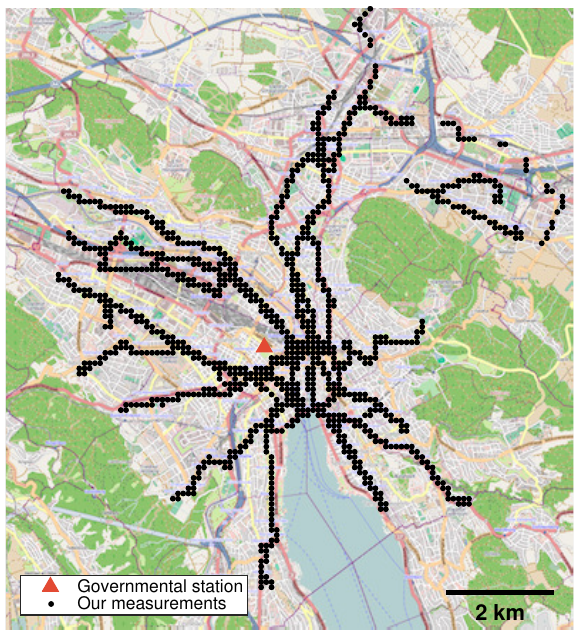
\includegraphics[scale=0.85]{imgs/ch_1/OpenSense_map_trams.png}
    \caption{OpenSense's stations in Zurich: ten public transport streetcars are equipped with a monitoring station; the dots denote locations with at least 50 measurements over the course of two years}
    \label{opensense_dots_zurich}
\end{figure}
\subsection{The station}
Being OpenSense a professional organization, they have been able to develop a far more efficient and reliable monitoring station than the proof-of-concept me and my colleagues built for the CINI Challenge 2018. Their stations are equipped with very good sensors and are also really well engineered in order to avoid water and dust entering the stations, see Figure \ref{opensense_station}.

Each station is operating when its streetcar is active, so on average 20h per day; typically from 1:00 AM to 5:00 AM the streetcars are off so no measurements are taken. All data is transmitted via a GSM module to the cloud, it's also important to notice that the stations buffer the data for a fixed amount of time, after that time has passed it sends a mean value of the gathered measurements.
\newline
\newline
For a complete and in depth explanation of how the stations work (how data is pre-processed before being sent to the cloud, what specific sensors are used) the reader can refer to the paper "Deriving High-Resolution Urban Air Pollution Maps Using Mobile Sensor Nodes" \cite{Deriving-High-Res-Maps}, a paper upon which I based my entire work. 

\begin{figure}[ht]
    \centering
    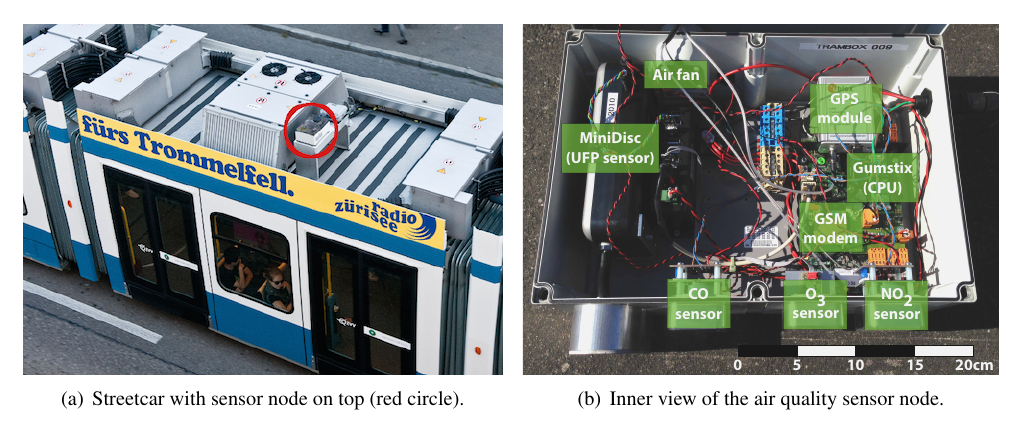
\includegraphics[width=\textwidth]{imgs/ch_1/OpenSense_station.png}
    \caption{(a) the stations are mounted on top of streetcars. (b) Inner view of the station, equipped with $UFP$, $CO$, $O_3$, $NO_2$ sensors, a GPS module and a GSM module}
    \label{opensense_station}
\end{figure}


\chapter{Work description}
The ultimate goal of this project is to have high-resolution pollution maps, in order to give a city's government to know exactly how the air quality is, in the most detailed fashion possible.
\newline
\newline
As CleanAir Project we have a really big limitation: cheap monitoring stations can be a really good ally in monitoring air quality, but the measurements are made with far too imprecise sensors therefore aren't usable in a legal way.

This means that if a station always measures too high levels of pollution near a specific building (e.g. a productive site of a company) the gathered data cannot be used in a court, the council cannot press charges. Therefore rather than being an instrument of maximum precision \textit{CleanAir aims at being a support tool in decision making for the planning of city-wide strategies against pollution}. 
\newline
\newline
Being this a rather unexplored field, there weren't too much studies already completed when I started working on this project; only the OpenSense Project in Zurich had a publicly available dataset tailored exactly for my needs, therefore I based my work on them, in order to have a comparison possibility against such a trustworthy study.

In this chapter both the OpenSense approach and the CleanAir one are presented.

\section{OpenSense approach}
The researchers in OpenSense proposed a complete method to produce high resolution pollution maps over Zurich \cite{opensense} specifically for Ultrafine particles (UFPs), which are particles with a diameter of less than 100nm; in ambient air the UFPs are mainly man-made as bioproducts of specific high temperature processes such as a car engine running.
\newline
\newline
They propose an approach based on mobile monitoring stations in order to enhance the spatial resolution by trading off temporal resolution. The basic idea is the same as CleanAir Project: \textit{a fleet of mobile monitoring stations can cover a large area without the need of a lot of stations}.

They deployed ten monitoring stations and put them on top of public streetcars for the city of Zurich, for a more detailed explanation on this regard take a look at \ref{opensense:intro}. 

\subsection{Data preprocessing}
\label{opensense:preprocessing}
Good data quality is a must for the development of reliable pollution maps, that's why the research group has put a lot of focus in preprocessing raw data by calibrating the sensors and filtering the results; Figure \ref{opensense_data_filtering} gives a graphical representation of the results of preprocessing and filtering the data.
\begin{figure}[ht]
    \centering
    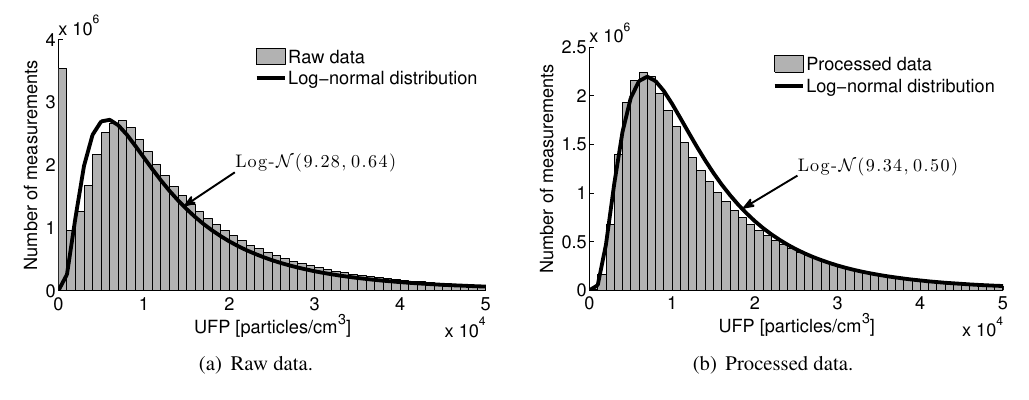
\includegraphics[width=\textwidth]{imgs/ch_2/OpenSense_data_filtering.png}
    \caption{(a) Raw data and their log-normal distribution. (b) Preprocessed and filtered data, the log-normal distribution now fits much better}
    \label{opensense_data_filtering}
\end{figure}
\newline
\newline
The actual process of validating the data is as follows:
\begin{enumerate}
    \item Analyze the statistical distribution of the monitored particles concentrations. usually ambient air pollutants closely follow a log-normal distribution (see Figure \ref{opensense_data_filtering}) Log-$N (\mu, \sigma^2)$.
    \item Evaluate the baseline signal of each device. They examine the correct offset of each MiniDiSCs (the pollution sensor) by looking at their baseline signals, \textit{i.e.} low-pass filtered measurements; a similar baseline signal is expected across all devices, because they take measurements in the same region. As baseline signal \textit{they take every 90 minutes} (the average time spent by a streetcar to cross the city twice) \textit{the 20th percentile of the measured concentrations}.
    \item Compare the produced measurements against the samples took by two high-quality stations in the same time period but in different locations in Switzerland. See Figure \ref{opensense_processed_vs_NABEL}.
\end{enumerate}
\begin{figure}[ht]
    \centering
    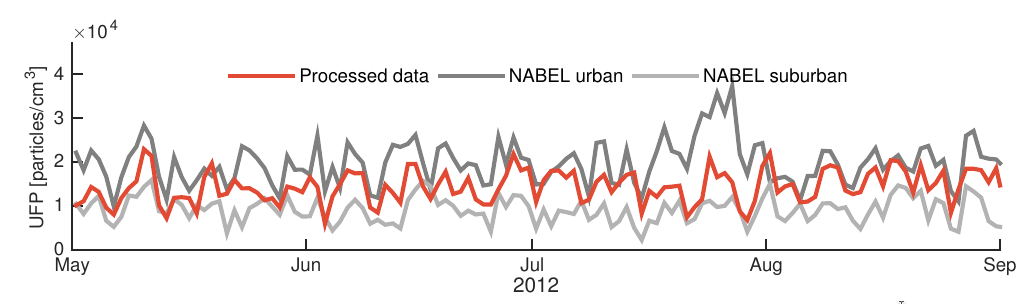
\includegraphics[width=\textwidth]{imgs/ch_2/OpenSense_processed_vs_NABEL.png}
    \caption{Daily average UFP concentrations measured by OpenSense in Zurich (red) against the two high-quality stations called NABEL at both urban (Pearson r=0.49) and suburban (r=0.55) locations} 
    \label{opensense_processed_vs_NABEL}
\end{figure}
In conclusion the corrected statistical distribution, the matching devices baseline signals and the good correlation between the processed data and the NABEL produced ones, guarantee a good quality of the processed data, therefore suitable to be used for producing accurate high-resolution pollution maps.
\subsection{Data aggregation}
\subsubsection{Temporal data aggregation}
The processed and filtered data are \textbf{aggregated in different time periods and for each time period a separate model is learned}, yielding to 989 models with yearly, seasonal, monthly, biweekly, weekly, daily and semi-daily (meaning from midnight to midday and vice versa) temporal resolutions.

\subsubsection{Spatial data aggregation}
The measured UFP concentrations are projected on a grid with 100m x 100m cells that completely covers Zurich. 

The measurements are unevenly distributed among 300-1300 different cells, depending on the analyzed temporal subset of the data; as an example in Figure \ref{opensense_dots_zurich} only the cells with at least 50 samples are showed, when projecting \textit{the full two-year data set on the grid}.
\subsection{Regression}
In order to create those high-resolution pollution maps the \textbf{Land-Use Regression models} (LUR) are a powerful ally, as they are widely used to asses spatial variation of air pollutants, typically at an intraurban scale \cite{lurmodels}.

LUR models use land-use informations and traffic characteristics (also called \textit{explanatory variables}) to predict pollution levels for location non covered by measurement devices; the general idea is as follows:
\begin{enumerate}
    \item At each measurement location (locations having an actual measurement device) the dependencies between the explanatory variables and the monitored pollutants are evaluated via linear regression.
    \item The relationships found in 1. are used to predict concentration levels at locations without measurement devices, but with available land-use data.
\end{enumerate}
The regression task is performed by a Generalized Additive Model (GAM) for it supports non-linear relationships between the monitored concentration levels and the explanatory variables and such models have been successfully used to analyze and model the spatio-temporal variability of particulate matter \cite{meteo-influence-pm}.

\subsubsection{Explanatory variables}
The researchers at OpenSense selected 12 explanatory variables, to be used with the LUR model, depicted in Table \ref{tab:explanatory_vars}.
\begin{table}[ht]
    \centering
    \begin{tabular}[p p]{l l}
         \hline
         Variable [unit] & Variable [unit]\\ [0.5ex] 
         \hline
         Population [inhabitants/ha] & Industry [industry buildings/ha]\\ 
         Building height [floor levels/ha] & Heating [oil and gas heatings/ha] \\
         Terrain elevation [average m/ha] & Road type [busiest road type/ha] \\
         Distance to next road [m] & Distance to next large road [m] \\
         Terrain slope [average degree/ha] & Terrain aspect [average degree/ha] \\
         Traffic volume [vehicles per day/ha] & Distance to next traffic signal [m] \\ [1ex] 
         \hline
    \end{tabular}
    \caption{Detailed list of the 12 explanatory variables used by OpenSense for their LUR model}
    \label{tab:explanatory_vars}
\end{table}
The variables related to the terrain (building heihgts, altitude, aspect of the terrain itself) are statistical estimates fetched from the Swiss Federal Statistical Office, while the variables related to streets (road type, distances to next roads, traffic signals) are extracted from OpenStreetMap. The average daily traffic volumes are obtained from the Department of Waste, Water, Energy and Air of the Canton Zurich.
\newline
\newline
Not all the variables have been used, due to their pair-wise correlation: \textit{removing variables that have high correlation with each other helps to better distinguish individual contributions of different variable to the predicted UFP value}. Both population density and number of gas and oil heating households are not used due to their high linear relationship with each other and with the number of floor levels. 

They also empirically found that using the distance to the next traffic signal didn't improve any of the models, so it isn't used.
\subsubsection{Generative Additive Model}
To actually predict the UFP concentration the following GAM is used:
\begin{align}
    ln(c_{num}) = a + s_1(A_1) + s_2(A_2) + \dots + s_n(A_n) + \epsilon
\end{align}
where $c_num$ denotes the UFP concentration, $a$ is the intercept, $s_1(A_1)\dots s_n(A_n)$ denote the smooth functions $s$ applied to the explanatory variables $A$, $\epsilon$ is the error term.
\newline
\newline
As for the GAM input, depending on the chosen temporal aggregation, \textit{only the $n$ cells with highest number of measurements are used} (for the full two-year data set the first 200 cells with highest number of measurements are used).

Usually those cells are the ones containing a tram stop, this ensures that the calculated means $c_i^m$ are reliable and provide a good trade-off between spatial distribution of the input and model perfomance. They empirically discovered that introducing prior weights to the cells did not bring any improvements to the model.
\begin{figure}[ht]
    \centering
    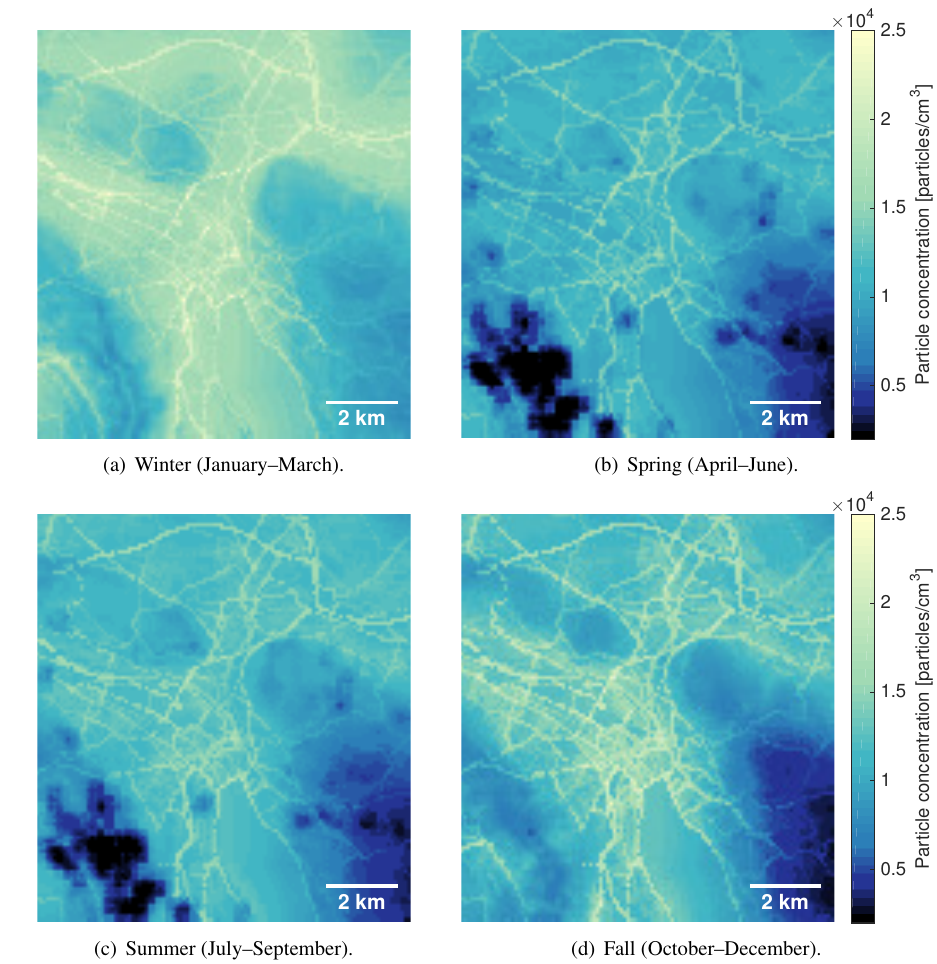
\includegraphics[width=\textwidth]{imgs/ch_2/OpenSense_heatmap.png}
    \caption{Output of the seasonal model, seasonal UFP concentration heatmaps with a spatial resolution of 100m x 100m} 
    \label{opensense_heatmap}
\end{figure}
\subsection{Model evaluation}
To evaluate the performance of the produced models the researchers of OpenSense use three standard metrics:
\begin{itemize}
    \item \textit{Factor of 2 measure (FAC)}. Quantitatively analyzes the scatter plots of predicted UFPs against the measured ones by evaluating the fraction of data points that lie inside the two factor area, which is the fraction of data that satisfies the following:
    \begin{align}
        0.5 \le \frac{c_i^P}{c_i^m} \le 2.0
    \end{align}
    where $c_i^P$ is the predicted value and $c_i^m$ is the measured one, all for the cell $i$ of the grid. This measure is used based on the assumption that an accurate model for pollution maps should have a relative scatter less than a factor of two. \cite{air-quality-evaluation}
    \item \textit{Root-mean-square-error (RMSE)}. Quantifies the difference between the predicted and measured particles concentrations, this metric is generally used when large errors are to prevent as much as possible, due to the error being squared:
    \begin{align}
        RMSE=\sqrt{\frac{\sum_{i=1}^N (c_i^P - c_i^m)^2}{N}}
    \end{align}
    \item \textit{Adjusted coefficient of determination ($R^2$)}. Indicates from 0 to 1 how well the predictions fit the measurements, meaning that having $R^2=1$ denotes a perfect fit. This measure reflects the linear relationship between the predicted values and the measured ones, hence, it's insensitive to additive and multiplicative errors.
\end{itemize}
\subsection{Application model}
\begin{figure}[ht]
    \centering
    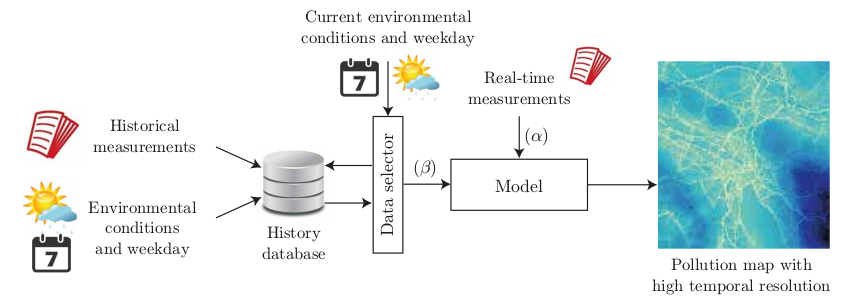
\includegraphics[width=\textwidth]{imgs/ch_2/OpenSense_data_flow.png}
    \caption{The complete conceptual model of OpenSense's application. Additional data from a database with historical measurements ($\beta$) is used to enhance the original dataset ($\alpha$). The data selector picks only historical measurements which were measured under similar (e.g. similar average condition in the modeled time period) environmental conditions are used. } 
    \label{opensense_flow}
\end{figure}
Figure \ref{opensense_flow} shows the complete conceptual model of the application produced by OpenSense; the history database is used to enhance the model capabilities on daily and semi-daily time periods, where the lack of data was inhibiting the model from performing well. Using this database reduced the RMSE by 26\% in said time periods.
\newline
\newline
The data selector is the key component to enhance the data set, because its job is to fetch historic measurements based on the average environmental condition of the modeled time period, which are the most likely to be similar to the real measurements of that time period.

They empirically decided which environmental variable to consider and how much fuzziness to concede to the selector, for example allowing $20\%$ of deviation on $15^{\circ}$ temperature means that the selector will return all measurements that have $15^{\circ} \pm 20\%$.

\section{CleanAir Project approach}
\label{cleanair:goals}
Having OpenSense's work as a baseline, I propose a different method to produce high-resolution pollution map given a fleet of mobile monitoring stations.
\newline
\newline
The proposed method uses a similar approach to the problem of data aggregation, but uses a Convolutional Neural Network to automatically extract the explanatory variables used by OpenSense and a Multilayer Perceptron to actually perform the predictions (instead of the Generalized Additive Model used by them).
\newline
\newline
The biggest challenge in data science is always about the data: having large amounts of good quality data is the \textit{conditio sine qua non} condition to solve a problem. In my case to have enough data was simply impossible, due to the fact that I only had one monitoring station and also at least a year of measurements is mandatory to let the system learn how seasons progress and relate to each other.

Thankfully I found about OpenSense's work and I have been able to download a complete year of measurements made by them, therefore with a wonderful spatial coverage and also a lot of already done pre-processing work (as explained in Section \ref{opensense:preprocessing}). 

\subsection{Network}
\label{cleanair:cnn_schema}
The Neural Network used to make the actual predictions is a slightly modified version of the traditional LeNet network (Figure \ref{lenet_schema}). 
\begin{figure}[ht]
    \centering
    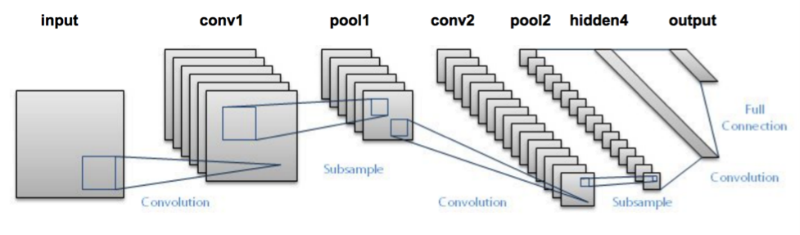
\includegraphics[width=\textwidth]{imgs/ch_2/LeNet_schema.png}
    \caption{The traditional LeNet convolutional network} 
    \label{lenet_schema}
\end{figure}
\begin{figure}[ht]
    \centering
    \includesvg[width=\textwidth]{imgs/ch_2/CleanAir_CNN_schema.svg}
    \caption{High-level schema of the implemented network, a slightly modified LeNet network} 
    \label{cleanair_cnn_schema}
\end{figure}
\newline
\newline
Figure \ref{cleanair_cnn_schema} shows a schema of the network used, the main principle is that \textit{given a portion of map and some weather data, we want to predict UFP concentrations}; now each component is presented.
\subsubsection{Convolutional Layers}
This is the part of the network in charge of automatically extracting the describing features of a given map. The basic idea is extracting unique explanatory variables for each cell, rather than using a fixed and static set of variables as OpenSense does.

We want to automatically generate those variables so that \textit{each portion of map has its own explanatory variables}, represented by the feature map produced by the Convolutional Layers.
\newline
\newline
Generally the main purpose of the convolutional layers in a CNN is the \textbf{feature extraction}, meaning that the kernels applied in those layers are adjusted in order to produce the most useful feature map for the given task (as explained in \ref{convolution:explanation}). 

In this context, the kernels applied are adjusted to obtain a feature map that sufficiently describes a geographical area, which is the image of the map provided in input.
\subsubsection{Weather MLP}
A separate Multilayer perceptron is built just for the weather data, in order to give to the system the ability of weighting each of them in possibly a really complex way.
\newline
\newline
It is a simple MLP with 8 inputs and 8 outputs and 4 hidden layers; after some experiments I found that enhancing the complexity of this perceptron doesn't bring that much improvements to the model's capabilities. 
\subsubsection{Bilinear Layer}
The fundamental block of this network is this layer: it applies a bilinear combination to two inputs of any shape. It is often used to combine two different convolution streams in single feature map, for CNN used in classification tasks.
\newline
\newline
The function applied is the following:
\begin{align}
    y = x_1^t A x_2 + b
\end{align}
where $x_1$ is the feature map produced by the convolutional layers and $x_2$ are the weighted weather data coming from MLP-1; $A$ and $b$ are learned, giving the model the ability to learn how to combine the map with the weather data in the best way.
\newline
\newline
The fundamental problem that was keeping the model from learning properly was that each cell is used more than one time (for example, in a daily time frame each cell holds 7 samples, so it will pass through the network 7 times) and therefore the final Multilayer perceptron would see the same image over and over, with only the weather data and the label to predict actually changing. Given that a 128x128 pixels image is actually a matrix of 128x128 values, and the weather data set has 8 features, using a standard Linear layer would basically cause the weather features to have close-to-zero impact on the prediction.
\newline
\newline
By seeing the same map portion with only varying weather data, the model wasn't able to learn enough correlations to actually predict the UFP value. With the introduction of this Bilinear layer, each map image is combined with the weather data used, therefore if prediction is performed on a daily time frame for example, the model will see 7 sligthly different images for each cell.
\subsubsection{Final MLP}
The final Multilayer perceptron has the task of actually making the prediction about UFP concentrations based on the output of the Bilinear layer. It is a standard MLP with a much higher number of neurons than the weather one, in order to give as much flexibility as needed to the model.
\subsection{Data set}
The dataset used is made up by the following features:
\begin{itemize}
    \item \textbf{time}. Time index of the sample, depends on the chosen time period
    \item \textbf{num\_particles}. Concentration of UFP particles, the label to predict (UFP/$cm^3$).
    \item \textbf{cell\_id}. Unique integer value, identificative for a cell.
    \item \textbf{temperature}. Average temperature ($C^{\circ}$).
    \item \textbf{atm\_pressure}. Average atmospheric pressure (hPa).
    \item \textbf{humidity}. Average air humidity (\%).
    \item \textbf{wind\_direction}. Average wind direction, originally it was a nominal feature (a possible value could be "Wind blowing from the east") so it is transformed to numerical by assigning an integer value to every possible nominal value.
    \item \textbf{wind\_speed}. Average wind speed (km/h)
    \item \textbf{lat, lon}. Coordinates of this cell's center.
\end{itemize}
In the data made publicly available from OpenSense there wasn't any weather information, therefore I found a data set containing hourly measurements from a weather monitoring station in the center of Zurich and merged those two toghether.
\newline
\newline
The map images used have a resolution of 128x128 pixels and come from the OpenStreetMap API; the original images were 256x256 but for the sake of performance have been reduced, no further pre-processing is performed.
\subsubsection{Data aggregation}
\label{cleanair:data-aggregation}
The spatial aggregation of data is performed in the same way as OpenSense, I created a grid with 100m x 100m cells that covers Zurich and whenever a new measurement comes to the system is assigned to its covering cell, as explained in \ref{cleanair:apparch}.
\newline
\newline
The temporal aggregation of the data set is performed on fixed time periods: \textbf{daily, weekly, monthly, seasonal}; each cell has the information about average measurements for each time period, as a csv file (or table). 
\begin{itemize}
    \item Daily concentrations: 7 rows, average concentrations of each day of the week
    \item Weekly concentrations: 54 rows, average concentrations for each week of the year (the week zero is from 01/01 to 07/01)
    \item Monthly concentrations: 12 rows, average concentrations for each month
    \item seasonal concentrations: 4 rows, average concentrations for each season, the northern meteorological division is used to assign each measurement to a season (all seasons are exactly 3 months long, for example spring lasts from 01/03 to 31/05)
\end{itemize}
The entries of these tables are going to be the inputs for the neural network; no further adjustments are made because of the good pre-processing work already done by OpenSense team.
\newline
\newline
To further clarify how the data are aggregated let us consider an example, suppose that we want to create the daily concentrations table having the whole set of measurements belonging to a cell: all measurements took on a monday will be averaged in order to get the monday average concentrations, and so on for each day of the week.

\chapter{Methodologies and tools}
In this chapter all the technologies and frameworks used in this research are briefly presented (only the ones relative to the deep learning module of the application).

\section{Python as programming language}
The programming language used in this research is Python3.7, the last stable release of one of the most used programming languages in the world of data science.
\newline
\newline
The object-oriented nature of Python facilitates data scientists to execute tasks with better stability, modularity, and code readability. While Data Science is only a small portion of the diverse Python ecosystem, this language is rich with specialized deep learning and other machine learning libraries and popular tools like scikit-learn, Keras, TensorFlow and the one that I've used in this thesis, PyTorch. Undoubtedly, Python enables data scientists to develop sophisticated data models that can be plugged directly into a production system.
\newline
\newline
Thanks to its wonderful support to the most common data set file formats (CSV, JSON,...) it facilitates the work of data scientists, giving them the possibility to focus on developing the best model rather than being stuck on small problems such as having to write a procedure to parse a JSON file.
\newline
\newline
It also has some disadvantages: due to its extreme object oriented "mindset" it is hardly ever used in production ambient, because of the overhead that all the frameworks bring to the table. Most of the times this isn't a problem though, because usually a scientist would develop and train the model using python and only once the model is considered to be ready it gets translated to a more efficient language, such as plain C, because almost every major machine/deep learning framework is also available in more efficient languages.

\section{Technologies for data aggregation and analysis}
The data gathering process (meaning having a method to access the monitoring stations data) relies on the MQTT protocol and is out of the scope of this thesis. A brief description can be found in \ref{cleanair:apparch}.

\subsection{MongoDB}
\begin{wrapfigure}{l}{0.3\textwidth}
    \centering
    \includesvg[width=0.3\textwidth]{imgs/ch_3/MongoDB_Logo.svg}
\end{wrapfigure}
MongoDB \cite{mongodb} is a document based database, classified as NoSQL. It is designed with ease of development and mostly scaling in mind, therefore it is really suitable to Big Data applications, where the number of data to handle can grow exponentially.
\newline
\newline
In MongoDB a record is called \textbf{document}. A document is essentially a JSON object, therefore made up by "field:value" couples; each field may contain a single value, an array, another document or an array of other documents.
\newline
Documents are stored in \textbf{collections}, which are analogous to tables in SQL databases.

The fact of using this document based approach brings three main advantages:
\begin{itemize}
    \item \textbf{Documents correspond to native data types in many languages}. The JSON standard is available as a native data type in many of the modern languages such as JavaScript or Python (in the form of Dictionary, the Python's name for this kind of data type).
    \item \textbf{Embedded documents and arrays reduce the need for expensive joins}. Traditional SQL databases are based on relationships between tables, in order to avoid as much as possible redundancy of data; such an approach grants minimal storage requirements and thanks to the atomic transactions it also grants safety of data. In Big Data applications usually the most important requirement is the quickness of reading and writing to the database rather than the safety of atomic transactions.
    \item \textbf{Dynamic schema supports polymorphism}. MongoDB is known as a "schemaless" database, meaning that it does not force any kind of structure for the documents in a collection and therefore it is possible that a collection may contain documents with different structures; this approach mimics the object oriented programming languages.
\end{itemize}
The key features of MongoDB are the following:
\begin{itemize}
    \item \textbf{High Performance}. The embedded data models greatly reduce the need for I/O operations on the database, and the indexes enable the support for faster queries, also including keys from embedded documents. 
    \item \textbf{Rich query language}. Read and write operations (CRUD) are supported by a powerful query language, enabling clients to perform complex queries and automated data aggregations with ease.
    \item \textbf{High availability}. MongoDB's support for \textbf{replica sets} provides automatic failover and data redundancy, a replica set is essentially a cluster of servers mantaining the same database in multiple copies.
    \item \textbf{Horizontal scalability}. A core functionality is the horizontal scalability of MongoDB databases, thanks to \textbf{sharding} the data of a single database can be distributed in a cluster of servers.
\end{itemize}
\subsection{Pandas}
\begin{wrapfigure}{l}{0.3\textwidth}
    \centering
    \includesvg[width=0.3\textwidth]{imgs/ch_3/Pandas_logo.svg}
\end{wrapfigure}
As said in the official Pandas GitHub repository \cite{pandas}, Pandas is “a Python package providing fast, flexible, and expressive data structures designed to make working with “relational” or “labeled” data both easy and intuitive. It aims to be the fundamental high-level building block for doing practical, real world data analysis in Python. Additionally, it has the broader goal of becoming the most powerful and flexible open source data analysis / manipulation tool available in any language. It is already well on its way towards this goal.”
\newline
\newline
The two main data structures in Pandas are Series and DataFrames:
\begin{itemize}
    \item \textbf{DataFrame}. Array of 2 dimensions, rows and columns.
    \item \textbf{Series}. Array of 1 dimension, constitutes a single column of a DataFrame.
\end{itemize}
These structures have really complex mechanism that enable the users to interact easily with the data. Making operations such as selections, slicings, aggregations of any kind is almost as easy as handling a normal array in Python.
\newline
\newline
The only downside of Pandas is that all the flexibility and ease of use granted by such structures means that a lot of overhead data is used, such as really complex indexes. When performing I/O operations on large amounts of data Pandas can become really slow, mostly when handling tasks such as merging thousands of files togheter: each time a file is opened via Pandas a DataFrame is created.
To perform those kind of tasks a more direct approach is advisable, such as the library "csv" available as a native package in every Python installation, which is much lighter even though it doesn't grants the same capabilities.

\subsection{Matplotlib}
\begin{wrapfigure}{l}{0.3\textwidth}
    \centering
    \includesvg[width=0.3\textwidth]{imgs/ch_3/Matplotlib-logo.svg}
\end{wrapfigure}
One of the main jobs of a data scientist is often \textbf{data visualization}, which basically is the practice of visualizing data in graphs, icons, presentations and more. It is most commonly used to translate data stored in complex structures into digestible insights, in order to make it understandable also for a non-technical audience.
\newline
\newline
Matplotlib (\cite{plot}) is the most popular data visualization library in Python's ecosystem. It supports basically any kind of graphical representation, from simple line plots to really complex plots, made up by many subplots and/or multiple lines.

In my thesis I've used the \textbf{pyplot interface}, an interface to matplotlib with commands that strive to be similar to MATLAB ones.
\newline
\newline
I've chosen this interface due to the high availability of tutorials on the internet and furthermore to its simplicity, at the cost of being slightly more rigid than the original matplot library. 

\section{Technologies for Deep Learning}
\subsection{PyTorch}
\label{pytorch:intro}
\begin{wrapfigure}{l}{0.3\textwidth}
    \centering
    \includesvg[width=0.3\textwidth]{imgs/ch_3/PyTorch_logo_black.svg}
\end{wrapfigure}
PyTorch \cite{pytorch-home} is a machine learning framework that strives to accelerate the path from research prototyping to production development. It has been originally developed by Facebook for its services and open sourced in early 2017, but in a short time it has become really popular and used by companies such as Twitter or Salesforce.
\newline
\newline
It is a port to Python of the Torch deep learning framework which can be used for building deep neural networks and executing \textit{tensor computations}, Torch is based on Lua.

Essentially \textit{PyTorch is a Python package which provides tensors computations}, where \textbf{tensors} are multidimensional arrays (just like numpy's ndarrays) which can lay on the GPU memory, and offers a \textit{dynamic computation graph}, meaning that instead of using a predefined static graph PyTorch builds the computational graph via the \textbf{autograd} package, therefore it is possible to modify the network (e.g. the computational graph) during runtime.

\subsubsection{Tensors}
Deep Learning is essentially computations on tensors, which can be seen as \textit{generalizations of a matrix, that can be indexed in more than 2 dimensions}. Actually, matrices and vectors are special cases of torch.Tensors, where their dimension is 1 and 2 respectively, see Figure \ref{pytorch_tensor} for a graphical representation.
\begin{figure}[ht]
    \centering
    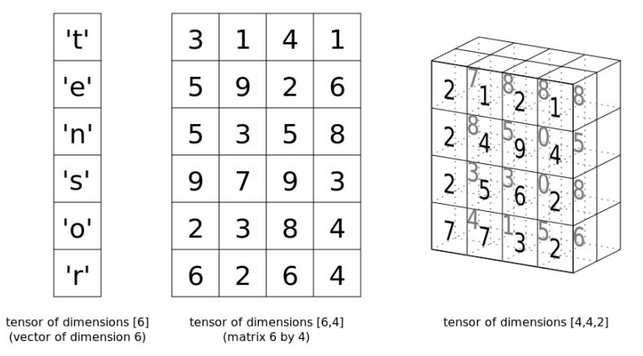
\includegraphics[width=\textwidth]{imgs/ch_3/pytorch_tensor.png}
    \caption{Tensors of different dimensions} 
    \label{pytorch_tensor}
\end{figure}
\newline
\newline
Tensors are really similar to NumPy's ndarrays, with the big addition of having the ability to reside on the graphics card memory and therefore highly enhancing the performances.

As said before, all computation in deep learning are essentially mathematical operations performed on data that may have more than one dimension. When said data is made up by images or audio the computations can become really heavy (think about multiplying two matrices of 256x256 elements, and such operation may be performed thousands and thousands of times to even finish one single experiment) so it becomes fundamental to accelerate the computation.

To do so tensors have been introduced: data structures able to reside on the GPU memory, so that all the computations can be performed by such piece of hardware, which is actually specialized in graphical computations, but performs very well nevertheless thanks to the fact that \textit{computations on images} (the job for which GPUs were invented) \textit{computations on images are exactly the same as tensors computations}: matrices operations have to be performed.
\subsubsection{Autograd package}
The concept of a computation graph is essential to efficient deep learning programming, because it allows the user to not have to write the back propagation gradients himself. \textit{A computation graph is simply a specification of how your data is combined to give you the output}.
\newline
Since the graph totally specifies what parameters were involved with which operations, it contains enough information to compute derivatives, and therefore lets the system automatically take care of writing the back propagation gradients and also enables the dynamic computation graph feature, one of the most important and distinctive features of PyTorch.
\newline
\newline
\textbf{Autograd} is the package in charge of keeping this mechanism working, and \textit{it is essentially a way of adding to each tensor of the model the information about how it was created}. To understand this concept let us consider an example: when two tensors are added together an output tensor is generated, but it has only the information about its data and its shape; if autograd is enabled on this object than the tensor will keep track of how it was created, so it will know what tensors created it and using what operation.
\newline
\newline
Generally speaking, autograd is an engine to automatically compute vector-jacobian product with the goal of automating the differentiation of each tensor: the backpropagation algorithm needs the derivatives of each tensor to work, therefore via autograd those derivatives are calculated each time the backpropagation runs, letting the user change the computation graph. For a detailed explanation see \cite{pytorch-autograd}.

Essentially it computes the sum of gradients of a given tensor, with respect to the graph leaves. The whole graph is differentiated using the \textbf{chain rule}, and the gradients are accumulated in the leaves.
\subsubsection{Object-oriented framework}
In 2019 PyTorch became the framework of choice at ICML \cite{icml} and many others important scientific conferences, stating its domain upon the scientific and academic communities.
\newline
\newline
PyTorch found its success mostly due to the fact that it tends to incline more towards Python when compared with any other library, therefore it is relatively easy to understand and it feels more natural, native and in line with Python code.
\newline
The Python nativeness of this framework means that it is built with object-oriented programming in mind, therefore even complex models are easily manageable and the actual code that implements them is relatively easy to understand, for those who are familiar with the object-oriented mindset.
\newline
\newline
Networks are implemented by means of the \textbf{nn.Module} interface, that requires only two methods:
\begin{itemize}
    \item \texttt{\_\_init\_\_()}: constructor method, where the structure of the network is defined. There are lots of different layers, activation functions, normalization layers, any kind of operation needed to implement deep neural networks.
    \item \texttt{forward(sample)}: defines how a sample passes through the network, each layer is essentially a method that requires a sample in input and outputs the result of its operation, such as \texttt{output = network.forward(sample)}.
\end{itemize}
\textbf{torch.utils.data.Dataset} is the data set interface, it defines how the data are read from memory and how a single sample is extracted from the data. It is up to the user of the Dataset class to decide how many samples extract at a time, what samples to extract, etc...
\newline 
Three methods are required:
\begin{itemize}
    \item \texttt{\_\_init\_\_()}: constructor method, where the data are read and kept in memory (a file \textit{.csv} could be read with Pandas library, the resulting DataFrame would be an attribute of the class Dataset).
    \item \texttt{\_\_len\_\_()}: returns the number of samples in the data set.
    \item \texttt{\_\_getitem\_\_(idx)}: given an index value \textit{idx}, this method returns the sample associated with that index. 
\end{itemize}
Once the Dataset and Network are defined the training script can be written quickly thanks to \textbf{torch.utils.data.DataLoader}, an utility that automates the process of querying the Dataset object for a sample. It provides lots of useful features such as multithreaded data loading and batch loading (extracting more than one sample at a time) that make the process of data loading as efficient and easy as possible.

\subsection{OpenCV}
\begin{wrapfigure}{l}{0.2\textwidth}
    \centering
    \includesvg[width=0.2\textwidth]{imgs/ch_3/OpenCV_Logo.svg}
\end{wrapfigure}
OpenCV \cite{opencv-docs} is an open-source BSD-licensed library that includes several hundreds of computer vision algorithms. It has a modular structure, meaning that it includes several shared or static libraries; the following modules are available:
\begin{itemize}
    \item \textbf{Core functionality}. It defines basic data structures used by the other modules.
    \item \textbf{Image Processing}. A module that includes algorithms to perform linear and non-linear image filtering, geometrical transformations, color space conversions, histograms, any kind of processing work that could be done on an image.
    \item \textbf{Video Analysis}. Automatic video analysis, including motion estimation, background subtraction and object tracking algorithms.
    \item \textbf{Camera calibration and 3D reconstruction, Object detection, \dots}.
\end{itemize}
Essentially OpenCV is a massive library used in almost any kind of Computer Vision task, thanks to the availability of lots of algorithms.
\newline
\newline
In the context of CleanAir Project, OpenCV has been used to preprocess the map images, and more specifically only to resize them from 256x256 to 128x128 pixels; no further manipulations have been needed, mostly because there wasn't any need for geometrical transformations or color space changings.
\chapter{Work description}
In this chapter I'll explain how I actually implemented all the functionalities discussed in \ref{cleanair:goals}.

\section{Statistical analysis}
Some simple statistical analysis have been performed on the data set before starting to aggregate the data, in order to deeply understand the actual feasibility of this research.
\begin{figure}[ht]
    \centering
    \includesvg[width=\textwidth]{imgs/ch_4/count_heatmap.svg}
    \caption{Heatmap describing the number of measurements per cell, before any kind of temporal aggregation} 
    \label{count_heatmap}
\end{figure}
\newline
\newline
First and foremost the number of measurements per cell has been analyzed, in order to have a high-level representation of the spatial coverage of OpenSense's stations after my own spatial aggregation. A heatmap has been produced (Figure \ref{count_heatmap}), due to the really high number of measurements in some cells (for example cells that include a tram stop have millions of samples, while cells without stops may have a few hundreds) the heatmap may seem to represent really sparse measurements, even if it isn't true.
\newline
\newline
\subsection{Correlation}
For each time frame the pair-wise correlation between the features of the data set has been analyzed, in order to check if there were features with too much correlation that would be useless for predictions.

\begin{table}[ht]
    \small
    \begin{tabular}{@{}l|llllllll@{}}
    \toprule
                & UFP     & temp.   & atm\_press. & humidity & wind\_dir. & wind\_speed & lat     & lon     \\ \midrule
    UFP         & 1.0     & 0.2873  & 0.0743      & 0.0743   & 0.0061     & -0.3747     & 0.0989  & -0.1074 \\
    temp.       & 0.2873  & 1.0     & 0.3324      & -0.7469  & 0.4611     & 0.0768      & -0.0422 & 0.2990  \\
    atm\_press. & 0.0743  & 0.3324  & 1.0         & -0.1791  & 0.1732     & -0.1793     & -0.1474 & 0.1656  \\
    humidity    & 0.0743  & -0.7469 & -0.1791     & 1.0      & -0.6254    & -0.3955     & 0.1394  & -0.0839 \\
    wind\_dir.  & 0.0061  & 0.4611  & 0.1732      & -0.6254  & 1.0        & 0.0538      & -0.1481 & -0.1199 \\
    wind\_speed & -0.3747 & 0.0768  & -0.1793     & -0.3955  & 0.0538     & 1.0         & -0.0584 & -0.0202 \\
    lat         & 0.0989  & -0.0422 & -0.1474     & 0.1394   & -0.1481    & -0.0584     & 1.0     & 0.1979  \\
    lon         & -0.1074 & 0.2990  & 0.1656      & -0.0839  & -0.1199    & -0.0202     & 0.1979  & 1.0     \\ \bottomrule
    \end{tabular}
    \caption{Correlation between features of the average Monday, from the daily time frame}
    \label{cleanair:correlation-table-monday}
\end{table}
\begin{table}[ht]
    \small
    \begin{tabular}{@{}lllllllll@{}}
    \toprule
                & UFP     & temp.   & atm\_press. & humidity & wind\_dir. & wind\_speed & lat     & lon     \\ \midrule
    UFP         & 1.0     & -0.2576 & 0.2016      & 0.1844   & -0.2861    & -0.2087     & 0.0111  & 0.0524  \\
    temp.       & -0.2576 & 1.0     & -0.6514     & -0.6457  & 0.4791     & 0.5379      & 0.3329  & -0.0164 \\
    atm\_press. & 0.2016  & -0.6514 & 1.0         & 0.1350   & -0.5018    & -0.5163     & -0.2556 & 0.0746  \\
    humidity    & 0.1844  & -0.6457 & 0.1350      & 1.0      & -0.5712    & -0.4980     & -0.3153 & -0.0132 \\
    wind\_dir.  & -0.2861 & 0.4791  & -0.5018     & -0.5712  & 1.0        & 0.7860      & 0.3905  & -0.0998 \\
    wind\_speed & -0.2087 & 0.5379  & -0.5163     & -0.4980  & 0.7860     & 1.0         & 0.3883  & 0.1017  \\
    lat         & 0.0111  & 0.3329  & -0.2556     & -0.3153  & 0.3905     & 0.3883      & 1.0     & -0.0531 \\
    lon         & 0.0524  & -0.0164 & 0.0746      & -0.0132  & -0.0998    & 0.1017      & -0.0531 & 1.0     \\ \bottomrule
    \end{tabular}
    \caption{Correlation between features of the average Week 1 of the year, from the weekly time frame}
    \label{cleanair:correlation-table-week1}
\end{table}
\begin{table}[ht]
    \small
    \begin{tabular}{@{}lllllllll@{}}
    \toprule
                & UFP     & temp.   & atm\_press. & humidity & wind\_dir. & wind\_speed & lat     & lon     \\ \midrule
    UFP         & 1.0     & 0.1283  & 0.1371      & 0.0821   & 0.0233     & 0.0244      & 0.0541  & -0.0102 \\
    temp.       & 0.1283  & 1.0     & 0.3771      & -0.7357  & 0.1667     & -0.1032     & -0.0070 & 0.0189  \\
    atm\_press. & 0.1371  & 0.3771  & 1.0         & -0.1989  & 0.7360     & 0.4406      & -0.4735 & -0.2923 \\
    humidity    & 0.0821  & -0.7357 & -0.1989     & 1.0      & -0.3371    & -0.1522     & -0.0158 & 0.2183  \\
    wind\_dir.  & 0.0233  & 0.1667  & 0.7360      & -0.3371  & 1.0        & 0.6383      & -0.2956 & -0.4918 \\
    wind\_speed & 0.0244  & -0.1032 & 0.4406      & -0.1522  & 0.6383     & 1.0         & -0.2296 & -0.3078 \\
    lat         & 0.0541  & -0.0070 & -0.4735     & -0.0158  & -0.2956    & -0.2296     & 1.0     & 0.1993  \\
    lon         & -0.0102 & 0.0189  & -0.2923     & 0.2183   & -0.4918    & -0.3078     & 0.1993  & 1.0     \\ \bottomrule
    \end{tabular}
    \caption{Correlation between features of the average January, from the monthly time frame}
    \label{cleanair:correlation-table-january}
\end{table}
\begin{table}[ht]
    \small
    \begin{tabular}{@{}lllllllll@{}}
    \toprule
                & UFP     & temp.   & atm\_press. & humidity & wind\_dir. & wind\_speed & lat     & lon     \\ \midrule
    UFP         & 1.0     & 0.3124  & -0.0716     & -0.1640  & 0.2223     & 0.2480      & -0.0227 & -0.1460 \\
    temp.       & 0.3124  & 1.0     & -0.2921     & -0.6826  & 0.4755     & 0.3550      & -0.1515 & -0.2490 \\
    atm\_press. & -0.0716 & -0.2921 & 1.0         & 0.2683   & -0.2173    & -0.1937     & -0.1199 & 0.0998  \\
    humidity    & -0.1640 & -0.6826 & 0.2683      & 1.0      & -0.7245    & -0.7507     & 0.1797  & 0.4412  \\
    wind\_dir.  & 0.2223  & 0.4755  & -0.2173     & -0.7245  & 1.0        & 0.5872      & -0.2843 & -0.4842 \\
    wind\_speed & 0.2480  & 0.3550  & -0.1937     & -0.7507  & 0.5872     & 1.0         & -0.0641 & -0.2435 \\
    lat         & -0.0227 & -0.1515 & -0.1199     & 0.1797   & -0.2843    & -0.0641     & 1.0     & 0.1991  \\
    lon         & -0.1460 & -0.2490 & 0.4412      & 0.4412   & -0.4842    & -0.2435     & 0.1991  & 1.0     \\ \bottomrule
    \end{tabular}
    \caption{Correlation between features of the average Winter season, from the seasonal time frame}
    \label{cleanair:correlation-table-winter}
\end{table}
The tables \ref{cleanair:correlation-table-monday}, \ref{cleanair:correlation-table-week1}, \ref{cleanair:correlation-table-january}, \ref{cleanair:correlation-table-winter} are representing the pair-wise correlation between all the features, including the label to predict, the UFP concentration. By looking at those tables some considerations can be made:
\begin{itemize}
    \item \textit{No feature should be eliminated}, in all time frames there aren't pair of features with too much correlation
    \item \textit{The correlation values arise as much as the temporal granularity arises}. The highest values of correlation can be found in the seasonal aggregation (\ref{cleanair:correlation-table-winter}), this is most likely due to the fact that by increasing the temporal granularity each period has much more measurements (the number of measurements took in a season is several orders of magnitude higher than the measurements took in a single day).
\end{itemize}
\subsection{Average UFP concentration analysis}
\begin{figure}[ht]
    \centering
    \includesvg[width=\textwidth]{imgs/ch_4/average_UFP_all_city.svg}
    \caption{The average UFP concentration for each time frame, average value for the whole city.} 
    \label{cleanair_average_ufp_city}
\end{figure}
Figure \ref{cleanair_average_ufp_city} shows the average UFP concentrations for each time frame. Such concentrations are obtained by setting a time index and then averaging all cell's concentration values, to further clarify let us consider an example: to have the average Monday from the daily time frame means setting considering only the average Monday for each cell and averaging those in the average Monday for the whole city of Zurich.
\newpage
\section{Data aggregation}
The very first problem to face was data aggregation, because it had to be performed on two levels: both a temporal and spatial, due to the fact that the data set has both a time index (the timestamp of each measurement) and a geographical index (the location in which the measurement was taken). 
\subsection{Spatial aggregation}
To aggregate the measurements spatially I followed the method used by OpenSense: a grid with cells of 100m x 100m that covers the whole city of Zurich.
\newline
\newline
OpenSense did not said how they built the grid, so I had to find my own method: 
\begin{enumerate}
    \item Define a square over Zurich by means of its south-west and north-east corners (in latlon format), said points are defined by me via OpenStreetMap's markers.
    \item From the south-west point add 100 meters to the east to find the next cell's center, repeat this process until the south-east corner is met.
    \item After a row is completed, from the south-east add 100 meters to the north to find the northern neighbour, then repeat step 2.
\end{enumerate}
With this algorithm I have been able to create the covering grid over Zurich, such grid is then saved as a collection in MongoDB, where the cells are the document of the collection.
\newline
\newline
After the grid was ready, the actual aggregation of data could be performed. The mechanism I choose to aggregate the data at the spatial level is simple: \textit{iterate trough the dataset, each measurement gets assigned to its belonging cell}, where a measurements belongs to a cell if the cell's center is the closest one to where the measurement was made.

The step of finding the nearest cell for a measurement is performed via the \textit{haversine formula} (\ref{haversine_formula}); the only problem left was that such a naive approach would require a really long time to conclude and therefore was not feasible for this project. That's why I decided to make use of MongoDB's powerful query mechanisms.
\newline
\newline
I saved both the grid and the dataset on MongoDB in separate collections, then I used the \textbf{\$geowithin} operator \cite{mongodb-geowithin}. It is a query operator focused on geographical queries, it selects all documents in a collection with geospatial data that exists entirely within a specified shape.

In this context the specified shape is the square represented by a cell, and the documents are all the measurements taken inside the "bounding shape".
\newline
\newline
There is only one constraint to use this operator: all the geospatial data has to be compliant to the GeoJson standard, which means respecting this format:
\begin{verbatim}
    {
        type: <GeoJSON type> , 
        coordinates: <coordinates>
    }
\end{verbatim}
A GeoJson type could be a Point, a LineString, or a Polygon. From the center of a cell its corners are calculated by subtracting 50 meters from each coordinate respectively, in order to form a Polygon.
\newline
\newline
By using this operator I was able to make use of the fantastic optimizations performed by MongoDB via its complex system of indexes.

\subsection{Temporal aggregation}
As explained in \ref{cleanair:data-aggregation} I choose a different approach than OpenSense, the dataset is first spatially aggregated and then averaged on these fixed time frames:
\begin{itemize}
    \item \textbf{Daily}: average day of the week, 7 measurements per cell.
    \item \textbf{Weekly}: average week, 54 measurements per cell.
    \item \textbf{Monthly}: average month, 12 measurements per cell.
    \item \textbf{Seasonal}: average season, 4 measurements per cell.
\end{itemize}
To perform this complex aggregations I made use of the powerful mechanisms offered by pandas (\cite{pandas-aggregation}), that are also strongly connected to the \textbf{datetime} library.

The connection with datetime has been fundamental, because pandas let me read the dataset and simultaneously parse the dates in it, so that manipulating said dates or accessing some parameters became really easy. 
\newline
\newline
Each time frame required the use of different mechanisms:
\begin{itemize}
    \item Daily: the \verb|datetime.day_name()| procedure returns the weekday of a given date, then aggregation is performed by weekdays.
    \item Weekly: the \verb|datetime.weekofyear()| procedure returns the week number of a given date, which is the order of the week, meaning that the week from 01/01 to 07/01 will be the week number 1.
    \item Monthly: every datetime object has attributes regarding the components of a date, so to access the month of a date is as easy as date.month.
    \item Seasonally: I choose to aggregate by metereological seasons, so I created a dictionary that associated every month with its season:
    \begin{verbatim}
        seasons = {
        1: 'WIN', 2: 'WIN', 3: 'SPR',
        4: 'SPR', 5: 'SPR', 6: 'SUM',
        7: 'SUM', 8: 'SUM', 9: 'AUT',
        10: 'AUT', 11: 'AUT', 12: 'WIN'
    }
    \end{verbatim}
    The aggregation is then performed by extracting the month of a date and associating that month with its corresponding season.
\end{itemize}


\section{Regression with Convolutional Neural Networks}
The framework used to build, train and evaluate the Convolutional Neural Network described in \ref{cleanair:cnn_schema} is PyTorch. 

\subsection{Creation of PyTorch.Dataset}
\subsection{Training}
\subsection{Evaluation}

\chapter{Conclusions and future developments}
\section{Results discussion}
\section{Future developments}

\printbibliography[heading=bibintoc,title={Bibliography}]



\end{document}